\documentclass[11pt]{article}
\usepackage[margin=0.85in]{geometry}
\usepackage[T1]{fontenc}
\usepackage{lmodern}
\usepackage{amsmath,amssymb,graphicx,booktabs,longtable,array}
\usepackage{hyperref,url,listings}
\hypersetup{colorlinks=true,linkcolor=blue,urlcolor=blue,
pdftitle={Independent double-difference tomography reconstruction}}
\lstset{basicstyle=\ttfamily\scriptsize,breaklines=true,columns=fullflexible}
\graphicspath{{../figures/}}
\title{An independent double-difference tomography implementation:\\synthetic reconstruction and limits of manuscript reproduction}
\author{Independent computational reproduction}
\date{October 2026}
\begin{document}
\maketitle
\begin{abstract}
Double-difference tomography uses paired seismic arrivals to reduce shared
travel-time errors while estimating source locations and velocity jointly.
Here we implement this inverse problem independently in C++ and test it
against the written model of Zhang and Thurber (2003). The code combines
variational ray tracing, trilinear velocity interpolation, joint linearization,
and damped, smoothed least squares. We reconstruct the specified synthetic
velocity profile and generate new event and station geometries. Consequently,
the true-model panel is independently reproduced, whereas synthetic inversion
panels are partial reproductions. The Hayward field-data figures depend on
observations excluded by the project instructions and are not reproduced.
All numerical figures in this report use saved output from this implementation.
The result is a reproducible method investigation, not a recovery of the
published Hayward velocity model.
\end{abstract}

\section{Scientific scope and evidence}
The target paper is Zhang and Thurber (2003), \emph{Bulletin of the
Seismological Society of America} 93, 1875--1889,
\href{https://doi.org/10.1785/0120020190}{doi:10.1785/0120020190}.
Its written equations, experiment descriptions, and captions are the scientific
specification. The publisher page returned HTTP 403; the complete manuscript
transcription posted by an author on
\href{https://www.researchgate.net/publication/215754286}{ResearchGate}
provided the text. No original model code, source observations, synthetic
arrival files, plotting scripts, or figure files were consulted or used.
No published plot was digitized. No published image appears in this report.

The exclusion of source observations has a direct scientific consequence.
A physical forward model can generate new arrival times for a specified
geometry, but it cannot recover the historical earthquake realization and
picking errors from a prose description. We therefore separate a reconstructible
velocity specification, an independent synthetic inverse experiment, and
unavailable field-data inversions. The panel audit preserves all eleven
manuscript figures rather than replacing the missing field results with
invented observations. No supplement is listed for this article on the original SSA issue contents
or its original abstract page. No supplementary figures were identified.
The official issue contents marks supplements for other articles explicitly;
\path{reference/specification_notes.md} records those checks.

\section{Forward problem and joint inversion}
Assume an isotropic, stationary medium and high-frequency geometric P rays.
Coordinates are in km, velocity in km/s, and time in s; depth is positive
downward. The predicted arrival of event $i$ at station $k$ is
\begin{equation}
 T_{ik}=\tau_i+\int_{\Gamma_{ik}}\frac{1}{v(\mathbf{x})}\,ds.
\end{equation}
Here $\tau_i$ is origin time and $\Gamma_{ik}$ is a stationary travel-time
path with fixed endpoints. The calculation includes no reflected or converted
phases, attenuation, or wave-amplitude effects. Paths remain inside the
rectangular model domain. There are no periodic or reflecting boundary
conditions.

Nodal velocities $v_n$ are interpolated trilinearly. Write the update as
$q_n=\delta\log(1/v_n)$, so that the nonlinear velocity update is
$v_n^{\rm new}=v_n\exp(-q_n)$. The absolute residual linearization is
\begin{equation}
 r_{ik}\simeq\mathbf{g}_{ik}\cdot\delta\mathbf{x}_i+
 \delta\tau_i+\sum_n K_{ikn}q_n,\qquad
 K_{ikn}=v_n\int_{\Gamma_{ik}}\frac{w_n(\mathbf{x})}{v(\mathbf{x})^2}\,ds.
\end{equation}
$w_n$ is the interpolation weight. The source derivative $\mathbf{g}_{ik}$
is evaluated from the differentiated endpoint segment integral. Absolute
arrivals constrain structure outside clusters and the common source shift.

For a measured event-pair difference $d_{ijk}$ at a common station, use
\begin{equation}
 r_{ijk}^{\rm DD}=d_{ijk}-(T_{ik}-T_{jk}),\qquad
 A_{ijk}^{\rm DD}=A_{ik}-A_{jk}.
\end{equation}
Velocity sensitivities from both events enter the difference, subject to
the 5 m sparsification rule described below. This includes changes in path
anomalies with source location. Shared station timing
errors cancel in differenced observations, whereas independent pick errors
do not. Catalog differences share errors with each other and with absolute
picks; our weighting follows the staged formulation without whitening this
covariance.

The linear step minimizes a weighted residual norm with first-difference
regularization of the final log slowness and damping of the column-scaled
increment. A first-difference row divides the difference between adjacent
nodes by their separation. Columns are normalized to unit Euclidean norm
before damping rows are added. An independently written LSQR implementation
solves the sparse system without forming normal equations. Absolute,
catalog-difference, and precise-difference rows receive stage weights
$(1,0.1,0.01)$, $(0.1,1,0.01)$, and $(0.001,0.01,1)$, respectively.
Smoothing and damping choices are explicit in the configuration. After a rejected update, identical repetitions within the same stage are skipped, while every later weight stage is retained.

Each accepted nonlinear step must decrease the current weighted misfit plus
roughness. Weights are frozen within that line search. Trial source locations
are projected onto the grid domain; velocities remain positive by logarithmic
parameterization. No published solution is used to choose an update. Sources
at boundaries and failed updates are counted in the results because they
can indicate model error or weak constraints.

\subsection{Ray integration and numerical substitutions}
The ray tracer minimizes discretized Fermat time with limited-memory BFGS
and Armijo backtracking, starting from a straight path. Each segment is split
at grid-plane crossings and integrated with two-point Gaussian quadrature.
This independent variational method replaces the paper's pseudo-bending
implementation. It searches for a local stationary path, with no guarantee
of finding every competing first-arrival branch. Search directions and
convergence gradients respect active model boundaries. Near-coincident
interior nodes are merged at a numerical tolerance far below ray spacing,
with the quasi-Newton history reset after such topology changes. Independent rays are traced
in parallel with OpenMP.

The reference configuration uses 1 km initial ray spacing and 180 ray
iterations, 18 nonlinear iterations in three equal stages, smoothing weight
5, and scaled damping 0.1. These choices are not all specified by the paper.
Distance and residual biweights, a 5 m differential path-coefficient cutoff,
regularization scaling, line search, and the residual-scale estimator are
fully defined in \path{METHODS.md} and the source. A damping or smoothing
number cannot be transferred between implementations without its scaling
convention. Our equal-direction gradient penalty should therefore not be
assumed identical to the original regularization.

\section{Independent synthetic experiment}
The true medium is constant with depth and along strike. Its cross-strike
profile is 6 km/s for $x\leq0$, falls linearly to 4 km/s at $x=1$ km,
remains 4 km/s through $x=5$ km, rises linearly to 5 km/s at $x=6$ km,
and increases linearly to 6 km/s at $x=38$ km. The paper describes sharp
gradients over $x=0$--1 and 5--6 km; linear interpolation across these two
transitions is our explicit assumption. Figure~\ref{fig:true} is generated
from saved model sampling and reconstructs the written velocity specification
with this assumption, without using published pixel values.

The inversion grid follows the coordinates in manuscript caption 2:
$x=(-35,-15,0,2,4,6,20,35)$ km,
$y=(-60,-40,-20,0,20,40)$ km, and
$z=(0,3,7,11,16)$ km. The forward grid adds the profile breakpoints
$x=1$ and 5 km. This prevents the data generator from using exactly the
same coarse representation as the inverse problem.

We generate 120 sources and 32 surface stations independently with seed
2003. Half the sources sample a 12 km wide region around the trough, and
half sample a broader 40 km interval; all sample the model volume in depth
and along strike. Stations use a jittered surface array. Figure~\ref{fig:geometry}
shows the complete generated geometry. These are not the paper's Loma
Prieta observations. The starting velocity is homogeneous at 5.5 km/s,
substituting for the paper's referenced layered starting model, whose values
are not tabulated in the target article. Independent starting source-coordinate
errors have standard deviation 0.6 km, with an initial depth restriction
of 0.5--15.5 km. Starting origin-time errors have standard deviation 0.05 s.

We round forward travel times to 0.01 s, add independent 0.04 s Gaussian
pick noise and a station-constant uniform bias between $-0.3$ and $0.3$ s.
Catalog differences subtract these noisy picks. Precise synthetic differences
subtract rounded forward times before added pick noise. This explicitly
resolves an ambiguity in the text's noise ordering in favor of precise
pair differences. Every event is observed at every station, and pairs within
20 km are selected. The saved arrival table separates exact time, rounding,
station bias, pick noise, and final observed time.
Subtracting two separately rounded arrivals permits differential rounding
errors approaching 0.01 s. The paper quotes 0.005 s for its differential
data; this discrepancy remains a limitation of our explicit rounding order.

\subsection{Starting-model sensitivity}
The target paper does not identify a side of the Dietz--Ellsworth model.
USGS Open-File Report 93-578, Table 4, tabulates two gradient adaptations
attributed to that work. We sample each named profile (LOM and LON) onto
the same inversion-depth grid and repeat DD inversion using otherwise
identical inputs. The adaptation footnote prevents identifying either as
the confirmed target start. This comparison measures sensitivity to two
written alternatives without inventing their values.
\begin{table}[htbp]\centering\small
\begin{tabular}{lrrrrr}\toprule Start & Median 3D error & Mean $|\Delta v|$ & Interior $|\Delta v|$ & $R_{\rm abs}$ & $R_{\rm prec}$\\\midrule
Homogeneous & 0.8222 & 0.3050 & 0.2135 & 0.3526 & 0.4390\\
LOM & 1.4316 & 0.4036 & 0.2589 & 0.3752 & 0.4370\\
LON & 1.1469 & 0.3606 & 0.2444 & 0.3780 & 0.4348\\
\bottomrule\end{tabular}

\caption{Starting-model sensitivity of the independent DD experiment.
LOM and LON are written gradient adaptations in USGS OFR 93-578.
All runs share geometry, true velocity, and observation noise. Median
three-dimensional location errors are in km, mean absolute velocity errors
are in km/s, and arrival residual RMS values are in s. The first velocity
column uses all saved slices; the interior column restricts $x$ to
$[-15,20]$ km, $y$ to $[-40,20]$ km, and depths to 3--11 km.}
\end{table}


\begin{figure}[p]\centering
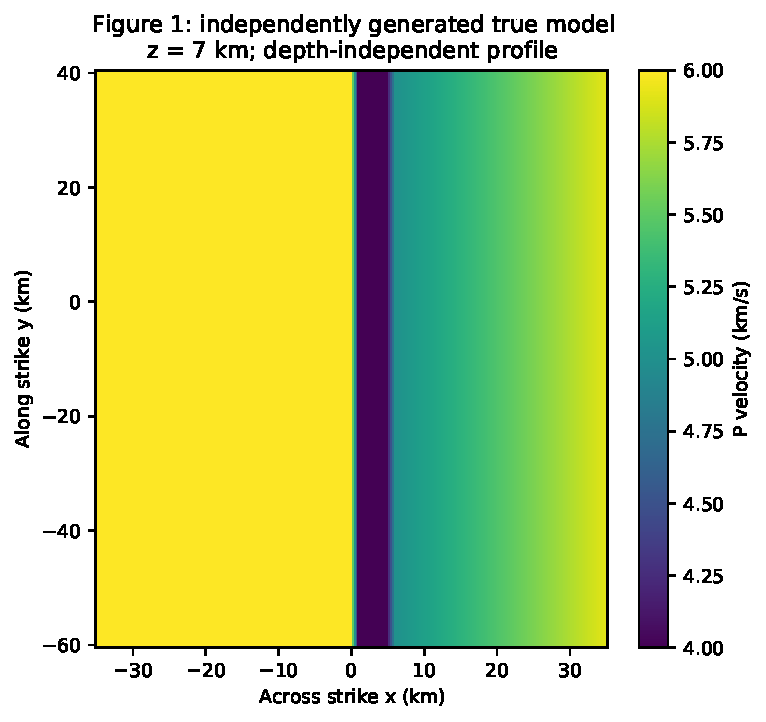
\includegraphics[width=0.73\textwidth]{figure01.pdf}
\caption{Manuscript Figure 1 reconstruction: true P velocity from the written
sandwich profile, sampled at 7 km depth. The model is independent of depth;
colors show velocity in km/s. All plotted samples are saved C++ output.
The trough occupies $x=1$--5 km and has velocity 4 km/s.}
\label{fig:true}\end{figure}
\begin{figure}[p]\centering
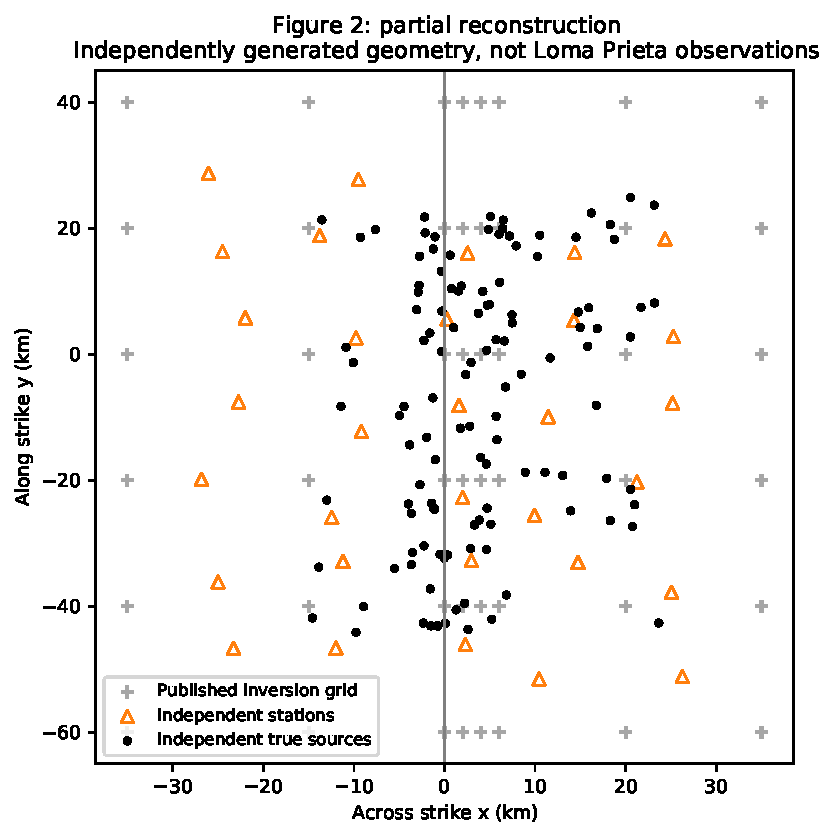
\includegraphics[width=0.78\textwidth]{figure02.pdf}
\caption{Partial reconstruction of manuscript Figure 2. Crosses are the
written inversion grid, triangles are independent stations, and dots are
independent true sources. The coordinates are experimental design choices,
not estimates extracted from the published map.}
\label{fig:geometry}\end{figure}

\section{Validation and numerical results}
All 32 implementation consistency checks passed. Across 32 deterministic source--receiver pairs, halving the ray segment spacing and increasing the iteration limit changed travel times by a median of 0.054 ms and a maximum of 0.892 ms. This check does not establish global ray optimality.

In the small known-model recovery check, the median three-dimensional location error decreased from 0.3035 to 0.0343 km; the final absolute-time RMS was 0.0034 s. Only 0.01 s time quantization remains in this check.

Before the main inversions, the median three-dimensional source error was 1.0285 km. The homogeneous 5.50 km/s initial model had mean absolute velocity errors of 0.456 km/s over the full domain and 0.544 km/s in the interior, evaluated at the same saved slice samples as the recovered models.

The standard run ended with median three-dimensional source error 1.7069 km, 0 sources on a model boundary, 1 zero-update iterations, and nodal velocities ranging from 2.41 to 7.05 km/s. LSQR converged in 10 of 10 solves, with worst relative normal residual 8.35e-09.
The dd run ended with median three-dimensional source error 0.8222 km, 0 sources on a model boundary, 1 zero-update iterations, and nodal velocities ranging from 3.74 to 6.41 km/s. LSQR converged in 18 of 18 solves, with worst relative normal residual 8.5e-09.
The loc1d run ended with median three-dimensional source error 2.9856 km, 11 sources on a model boundary, 1 zero-update iterations, and nodal velocities ranging from 5.50 to 5.50 km/s. LSQR converged in 15 of 15 solves, with worst relative normal residual 9.64e-09.
The loc3d run ended with median three-dimensional source error 0.1974 km, 14 sources on a model boundary, 0 zero-update iterations, and nodal velocities ranging from 4.00 to 6.00 km/s. LSQR converged in 18 of 18 solves, with worst relative normal residual 9.32e-09.


Relative to standard tomography, DD changed the full-domain mean absolute velocity error by -0.269 km/s and the median depth error by -0.996 km. Negative differences indicate improvement. These comparisons refer only to the independent experiment.

The analytic homogeneous joint-inversion recovery gates \textbf{PASSED}. Median three-dimensional location error changed from 0.1821 to 0.0210 km, while median velocity error at the 203 illuminated nodes changed from 0.3000 to 0.0080 km/s. The absolute residual RMS changed from 0.35209 to 0.00635 s. The precise residual RMS changed from 0.09192 to 0.00031 s. There were 12 accepted velocity updates, 12 accepted location updates, and 0 sources on a boundary. LSQR met its normal-residual tolerance in 12 of 12 solves; the worst relative normal residual was 9.15e-09.

The fixed recovery criteria require positive finite velocities, no boundary sources, nonincreasing accepted frozen-weight objectives, at least tenfold reductions of both absolute and precise residual RMS, lower median location and illuminated-node velocity errors, and nonzero updates to both locations and velocity. Illumination means accumulated interpolated path length greater than $10^{-9}$ km on final rays; it does not establish resolution or recovery at every node. The arrivals are analytic and unrounded. This test examines a coupled homogeneous limiting case; it does not establish heterogeneous model recovery.

Ray diagnostics compare production traces with half-spacing, 1000-iteration traces at the saved true, final standard, and final DD models and event locations. Source derivatives are compared with central differences of refined travel times using 0.01 km endpoint perturbations. A diagnostic exceedance uses the existing single-ray tolerance of 0.003 s/km; it is not a demonstrated inversion-error bound.

For the truth model, 32 rays had median and maximum absolute refinement changes of 0.054 and 0.892 ms. Production/refined convergence counts were 15/20 out of 32; maximum projected gradients were 0.00868/0.000668 s/km and maximum raw gradients were 0.00868/0.000668 s/km. Thus 17/12 production/refined traces failed the optimizer stopping criterion. Across 24 eligible source-coordinate derivatives, maximum production/refined errors were 0.000584/0.000599 s/km, with 0/0 components exceeding the diagnostic tolerance; 0 components were skipped at boundaries.

For the standard model, 32 rays had median and maximum absolute refinement changes of 0.155 and 0.684 ms. Production/refined convergence counts were 1/3 out of 32; maximum projected gradients were 0.0118/0.00645 s/km and maximum raw gradients were 0.0118/0.00645 s/km. Thus 31/29 production/refined traces failed the optimizer stopping criterion. Across 24 eligible source-coordinate derivatives, maximum production/refined errors were 0.000746/0.000328 s/km, with 0/0 components exceeding the diagnostic tolerance; 0 components were skipped at boundaries.

For the dd model, 32 rays had median and maximum absolute refinement changes of 0.100 and 0.861 ms. Production/refined convergence counts were 1/8 out of 32; maximum projected gradients were 0.0115/0.014 s/km and maximum raw gradients were 0.0115/0.014 s/km. Thus 31/24 production/refined traces failed the optimizer stopping criterion. Across 24 eligible source-coordinate derivatives, maximum production/refined errors were 0.000589/0.000179 s/km, with 0/0 components exceeding the diagnostic tolerance; 0 components were skipped at boundaries.

Raw and projected gradients differ at active domain boundaries. Small changes in travel time do not establish derivative convergence, and unconverged refined traces are not exact references. These deterministic samples cannot establish global first-arrival optimality or the accuracy of every production ray.

\begin{figure}[htbp]\centering
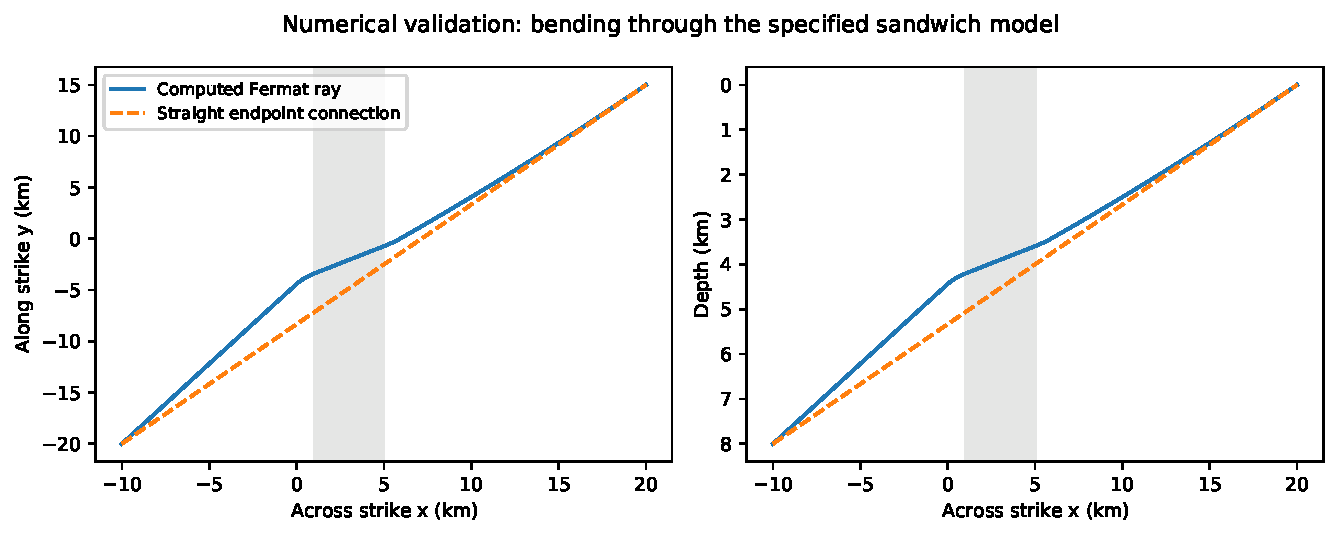
\includegraphics[width=\textwidth]{validation_ray.pdf}
\caption{Saved numerical ray through the specified sandwich medium, compared
with the straight connection between identical endpoints. The shaded region
marks the low-velocity trough. Bending reduces calculated travel time.
This is a validation figure, not a manuscript-panel reproduction.}
\end{figure}

The exact homogeneous travel-time solution, derivative checks, reciprocal
ray times, station-error cancellation, and known least-squares solution test
different parts of the implementation (Appendix~\ref{sec:validation}).
They do not establish uniqueness of the nonlinear inverse problem. A
larger, deterministic ray sample tests the production settings against
half-spacing, 1000-iteration traces. The source finite-difference checks are reported for both the true and
inferred media. Small travel-time differences alone do not establish
stationarity or accurate source derivatives. Raw gradients can also be
nonzero at active constraints, so projected gradients and iteration limits
are recorded separately. The homogeneous joint test generates arrivals
analytically as distance divided by 6 km/s, independently of the ray tracer,
and enables both source and velocity unknowns.

The cross-strike-only medium also admits an independent Snell-law reference
for the validation ray, which crosses the layers monotonically. If $R$ is
the endpoint separation in the transverse plane, its conserved transverse
slowness $p$ satisfies
\begin{equation}
 R=\int_{x_a}^{x_b}\frac{p\,v(x)}{\sqrt{1-p^2v(x)^2}}\,dx,\qquad
 T=\int_{x_a}^{x_b}\frac{1}{v(x)\sqrt{1-p^2v(x)^2}}\,dx.
\end{equation}
This scalar reference tests both travel time and the source slowness vector
without optimizing path vertices. At the 600-iteration setting, a
source-perturbation sweep found finite-difference errors below
$1.53\times10^{-4}$ s/km at 0.1, 0.03, and 0.01 km, while the 0.001 km
difference amplified ray-discretization and optimization errors to
0.00350 s/km. More iterations did not ensure finite-difference convergence.
The consistency check therefore uses
0.01 km, matching the larger ray diagnostic sample; the derivative tolerance
remains 0.003 s/km. The saved sweep in \path{data/development/} records this
limitation. It is not evidence of derivative convergence in every inferred
three-dimensional medium.

\begin{table}[htbp]\centering\small
\begin{tabular}{lrrrrrr}\toprule Method & Median $|\Delta x|$ & Median $|\Delta y|$ & Median $|\Delta z|$ & $R_{\rm abs}$ & $R_{\rm cat}$ & $R_{\rm prec}$\\\midrule
standard & 0.5232 & 0.4525 & 1.5176 & 0.3565 & 0.4621 & 0.4619\\
dd & 0.3690 & 0.3266 & 0.5217 & 0.3526 & 0.4399 & 0.4390\\
loc1d & 2.0050 & 0.5019 & 0.8753 & 0.6342 & 0.5095 & 0.5081\\
loc3d & 0.0103 & 0.0221 & 0.1955 & 0.1771 & 0.0578 & 0.0154\\
\bottomrule\end{tabular}

\caption{Independent synthetic results. Coordinate errors are in km and
arrival residual RMS values are in s. Residual RMS values are unweighted,
so they remain comparable when inversion weights change. Fixed-model
relocations are denoted loc1d (homogeneous) and loc3d (true synthetic grid).
These fixed-model comparisons retain absolute arrivals and do not copy all gauge conventions of hypoDD. The axes are Cartesian, not the latitude/longitude axes of published Table 1.}
\end{table}

\begin{table}[htbp]\centering\small
\begin{tabular}{llrrr}\toprule Method & Domain & Median & Mean & Standard deviation\\\midrule
Initial & Full domain & 0.500 & 0.456 & 0.318\\
Initial & Interior & 0.500 & 0.544 & 0.393\\
standard & Full domain & 0.443 & 0.574 & 0.506\\
standard & Interior & 0.258 & 0.313 & 0.245\\
standard & Published reference & 0.164 & 0.245 & 0.249\\
dd & Full domain & 0.252 & 0.305 & 0.262\\
dd & Interior & 0.153 & 0.214 & 0.181\\
dd & Published reference & 0.136 & 0.178 & 0.164\\
\bottomrule\end{tabular}

\caption{Absolute velocity errors in km/s. Full-domain statistics use saved
regular samples on all five depth slices. The interior restricts $x$ to
$[-15,20]$, $y$ to $[-40,20]$, and depths to 3--11 km. Published values
are reference scales only: the article does not specify the averaging mask,
and its geometry and starting model differ.}
\end{table}

\begin{table}[htbp]\centering\small
\begin{tabular}{lrrrr}\toprule Model & Depth (km) & Trough & West block & West minus trough\\\midrule
standard & 3 & 4.440 & 5.561 & 1.121\\
standard & 7 & 4.592 & 5.948 & 1.356\\
dd & 3 & 4.202 & 5.779 & 1.577\\
dd & 7 & 4.238 & 5.901 & 1.663\\
Specified true model & 3, 7 & 4.000 & 6.000 & 2.000\\\bottomrule\end{tabular}

\caption{Spatial recovery of the specified trough and western block. All
velocities and contrasts are in km/s. Arithmetic means use saved samples
with $y\in[-20,20]$ km, $x\in[1,5]$ km for the trough, and
$x\in[-15,0]$ km for the western block, including window endpoints.
These independently defined windows quantify recovery of the known 2 km/s
contrast; they are not published recovered-model averages.}
\end{table}

DD reduces the full-domain mean velocity error from the initial 0.456 to
0.305 km/s; standard tomography ends at 0.574 km/s. The DD value remains
larger than the published reference of 0.178 km/s, under the differing
sampling and starting conditions described above. Median three-dimensional
location error improves from 1.029 to 0.822 km with DD, although its median
depth error, 0.522 km, is slightly worse than the initial 0.477 km.
Thus improvement depends on both the quantity and the averaging domain.

The recovered DD western-block--trough contrasts are 1.577 and 1.663 km/s
at 3 and 7 km depth, respectively, compared with the specified 2 km/s.
DD preserves more contrast than standard tomography but still smooths the
trough. Its unweighted precise-difference RMS remains 0.439 s, compared with
0.462 s for standard tomography and 0.0154 s with the true velocity fixed.
The DD residual is far above the approximately 0.01 s upper bound on
differential rounding error: the nearly exact synthetic differences are
not fitted to their precision. Grid representation, regularization,
source--velocity trade-offs, and robust downweighting are possible
contributors; these experiments do not isolate their effects.
Improved model-error averages therefore do not imply a close fit to every
event pair. Among the three tested starting profiles, the homogeneous start
gives the smallest final location and velocity errors; this is a sensitivity
result for the independent experiment, not identification of the paper's start.
The LOM and LON runs end with median three-dimensional errors of 1.432 and
1.147 km, respectively, both worse than the initial 1.029 km.

All sampled travel-time refinement changes are below 0.9 ms, smaller than
the 10 ms rounding interval and 40 ms random-pick scale. None of the sampled
source derivatives exceeds the 0.003 s/km diagnostic tolerance. However,
most rays in the inferred models do not meet the stricter optimizer stopping
criterion, including many refined traces. These checks show close agreement
between the numerical settings on sampled paths. They do not certify
absolute accuracy, all derivatives, or the first-arrival branch selected
by every ray.

Each Figure 3 counterpart shows the five generated grid-depth slices at
0, 3, 7, 11, and 16 km. The published captions do not enumerate plotted
depths, so this count is not a verified reconstruction of the published
figure layout.

\begin{figure}[p]\centering
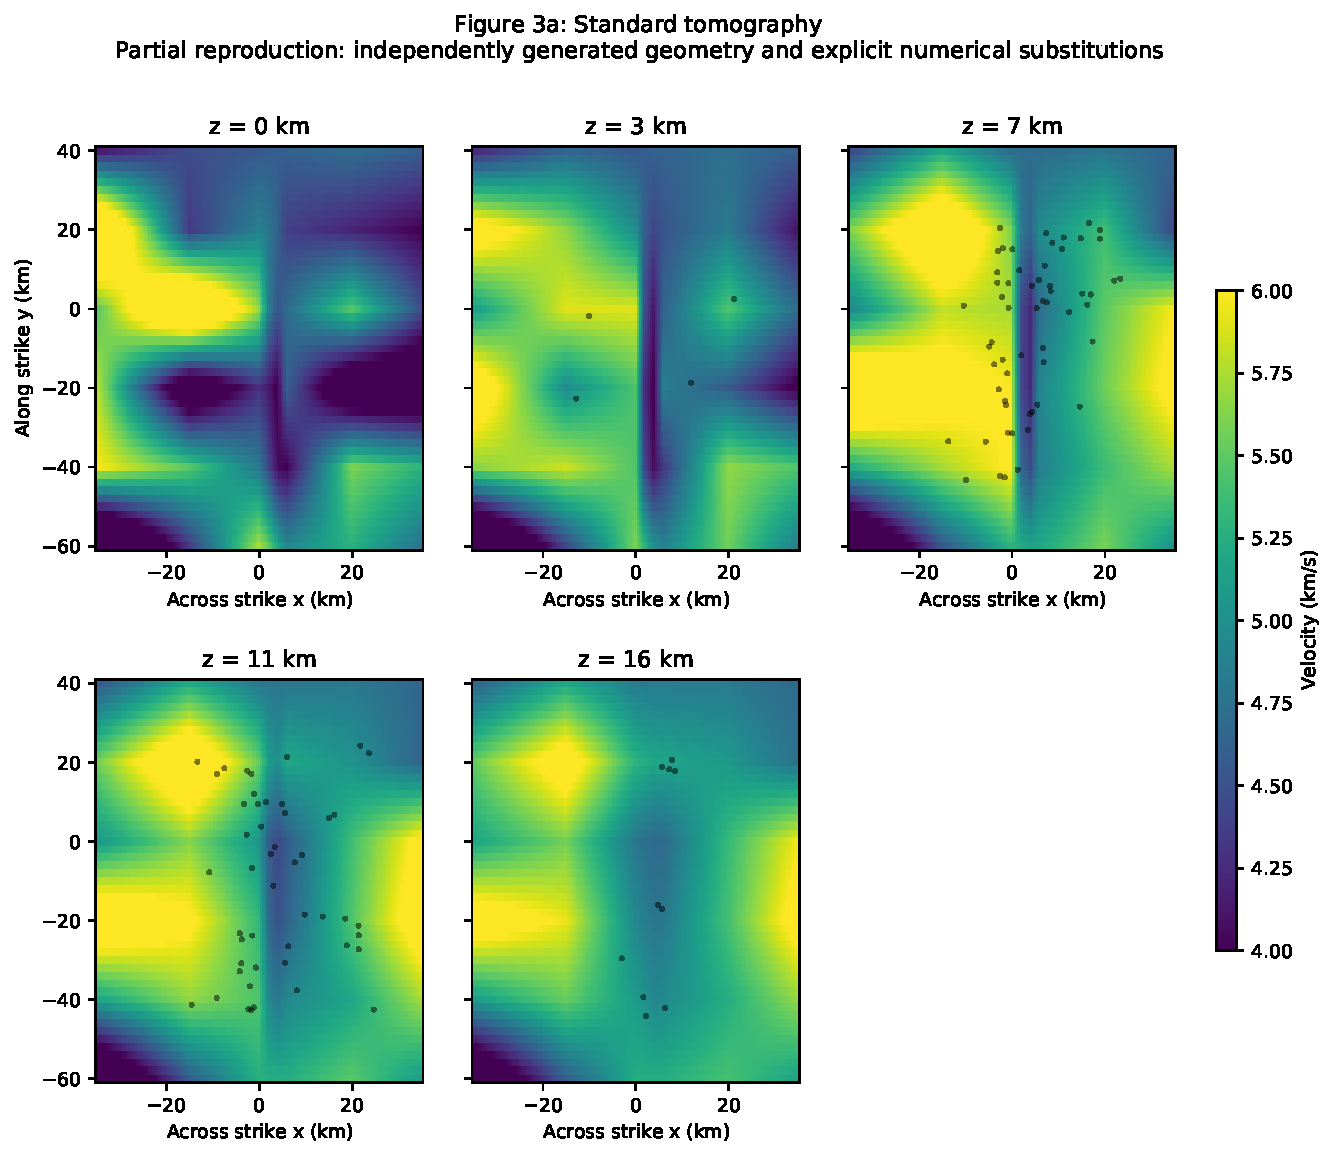
\includegraphics[width=\textwidth]{figure03a.pdf}
\caption{Partial reconstruction of manuscript Figure 3a: standard tomographic
velocity from independent observations. Dots are inferred sources selected
by adjacent depth midpoints. Colors show 4--6 km/s; values outside this
interval saturate and their numerical range is reported in the text.
Unconstrained boundaries must not be read as resolved structure.}
\end{figure}
\begin{figure}[p]\centering
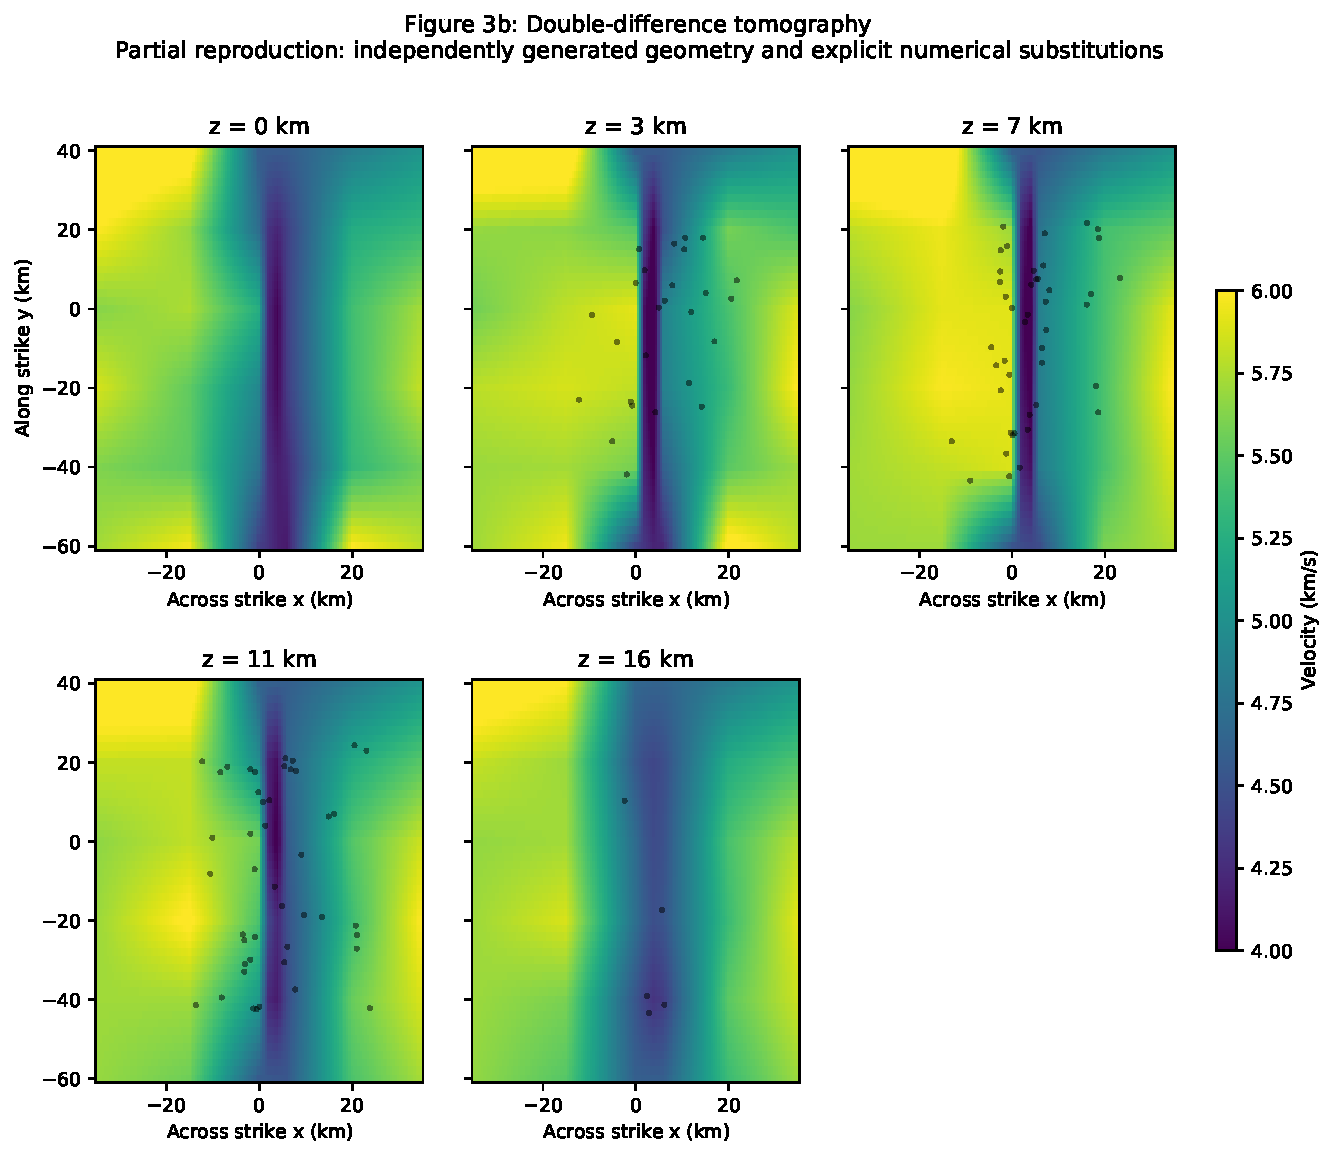
\includegraphics[width=\textwidth]{figure03b.pdf}
\caption{Partial reconstruction of manuscript Figure 3b: DD velocity from
independent observations. The initial model, true medium, noise, and inversion
grid are identical to those of the standard run. Colors and source-selection
conventions follow the preceding figure.}
\end{figure}
\begin{figure}[p]\centering
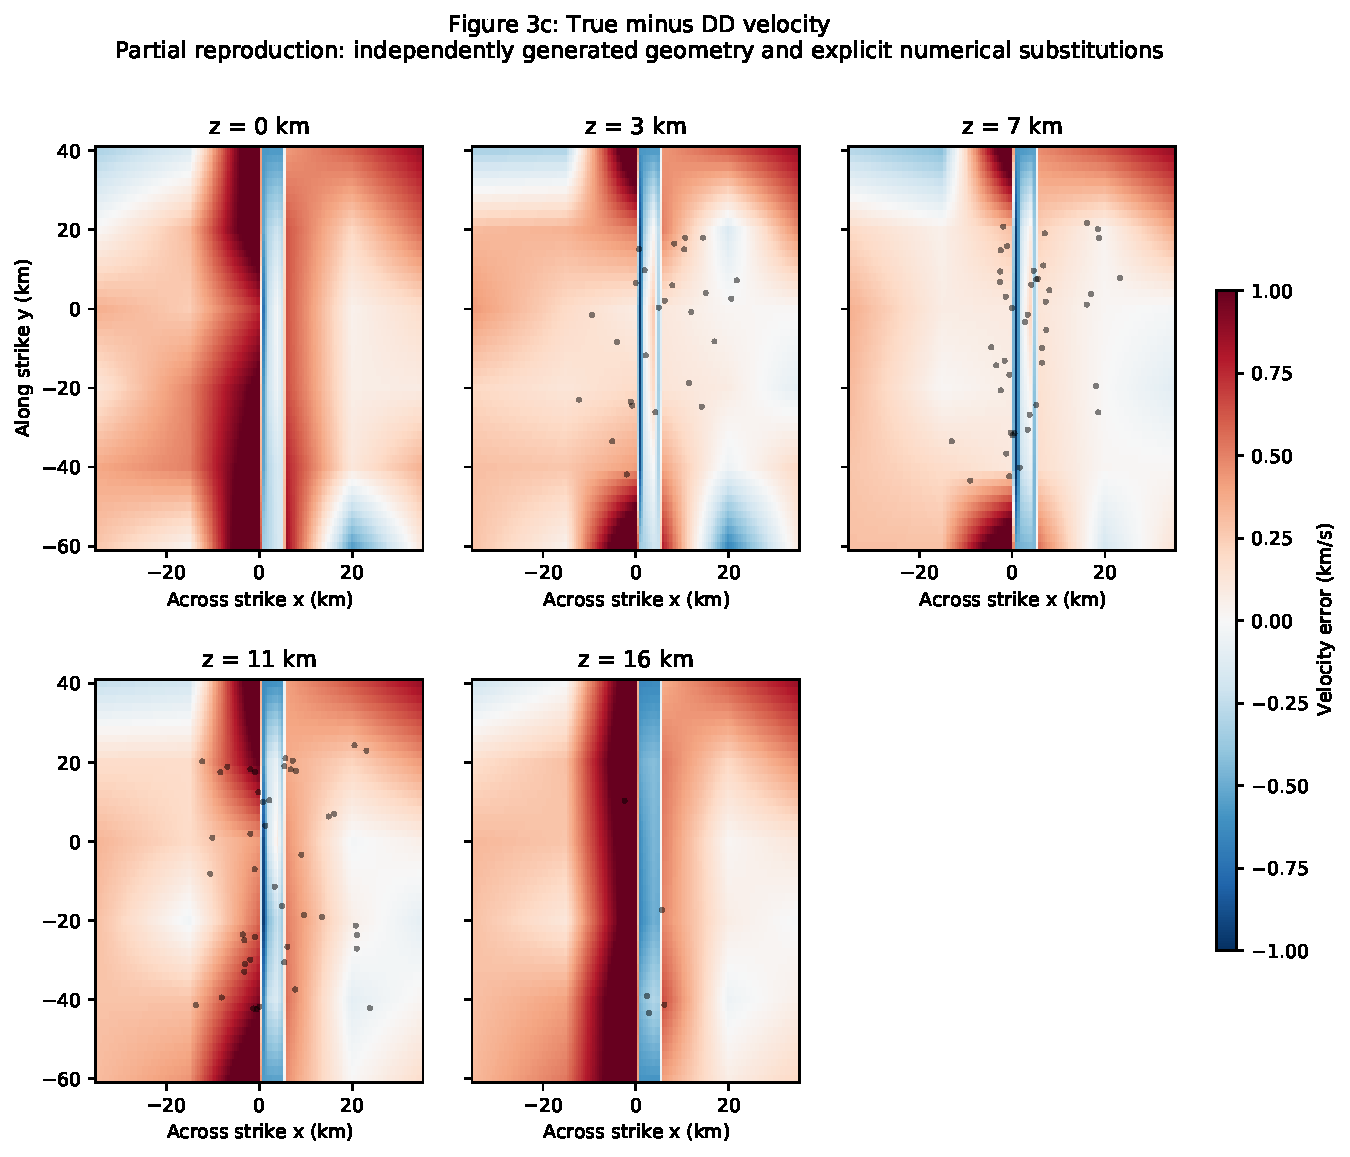
\includegraphics[width=\textwidth]{figure03c.pdf}
\caption{Partial reconstruction of manuscript Figure 3c: true minus DD
velocity, following the subtraction order in the manuscript's prose.
Blue marks recovered velocities that are too fast, and red marks recovered
velocities that are too slow. The fixed color range is $\pm1$ km/s. Saved samples retain
unsaturated values.}
\end{figure}
\begin{figure}[p]\centering
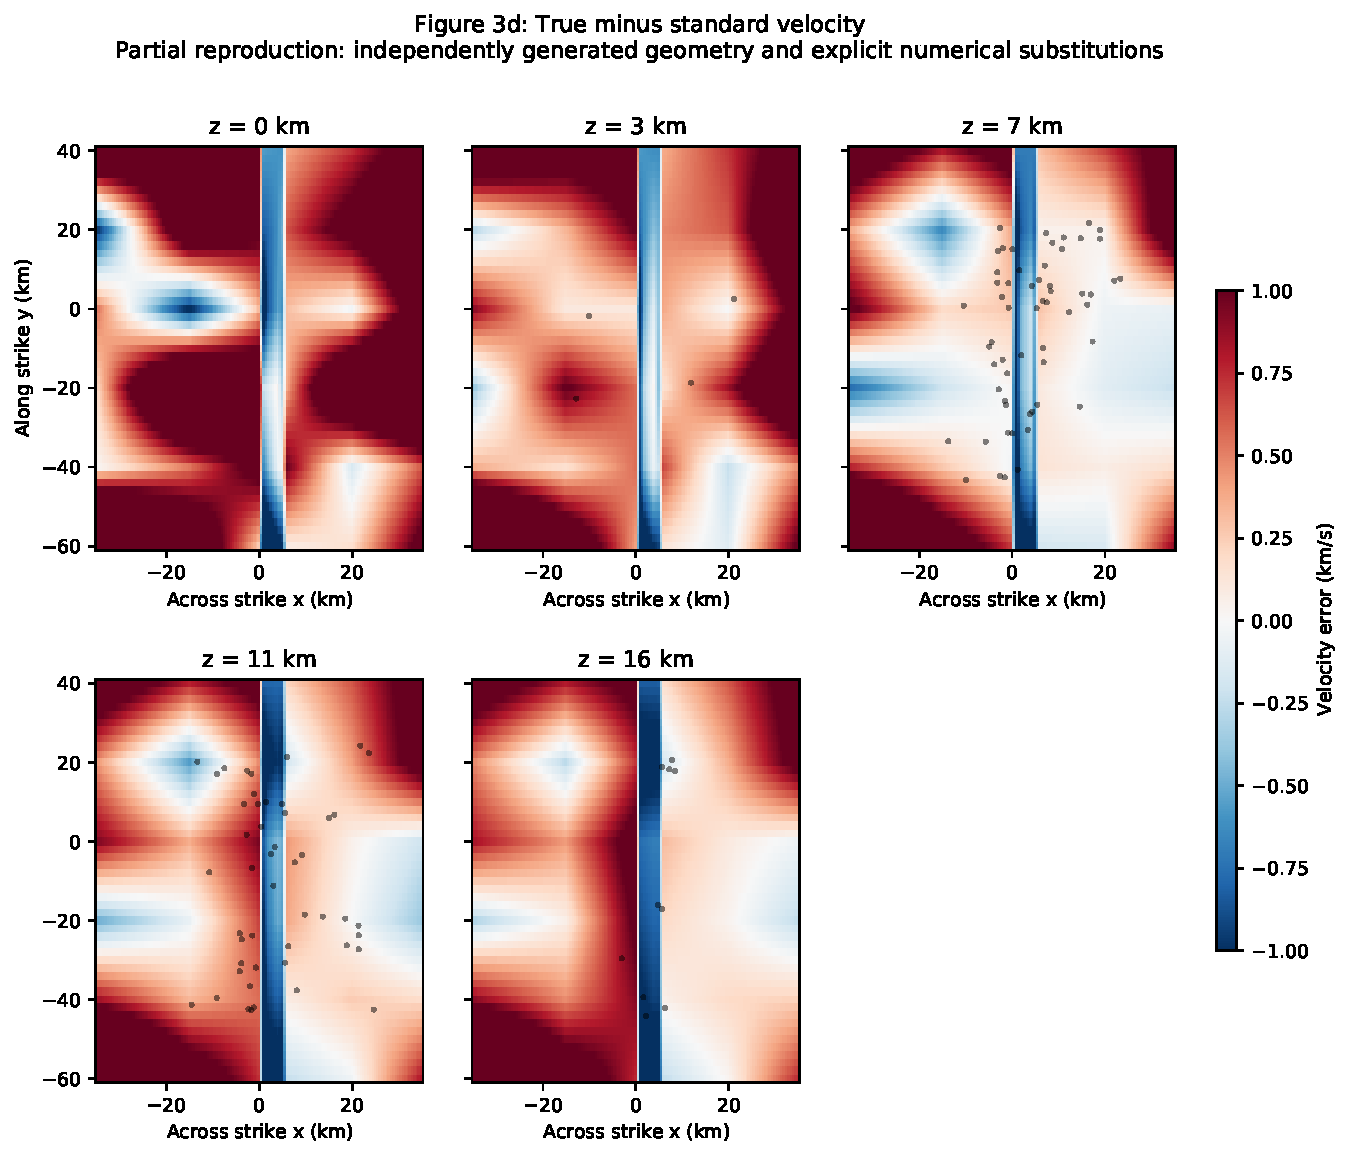
\includegraphics[width=\textwidth]{figure03d.pdf}
\caption{Partial reconstruction of manuscript Figure 3d: true minus standard
tomographic velocity, with the sign and color convention of the preceding
figure. The spatial patterns depend on the independent geometry and cannot
be compared point by point with the original inversion.}
\end{figure}
\begin{figure}[p]\centering
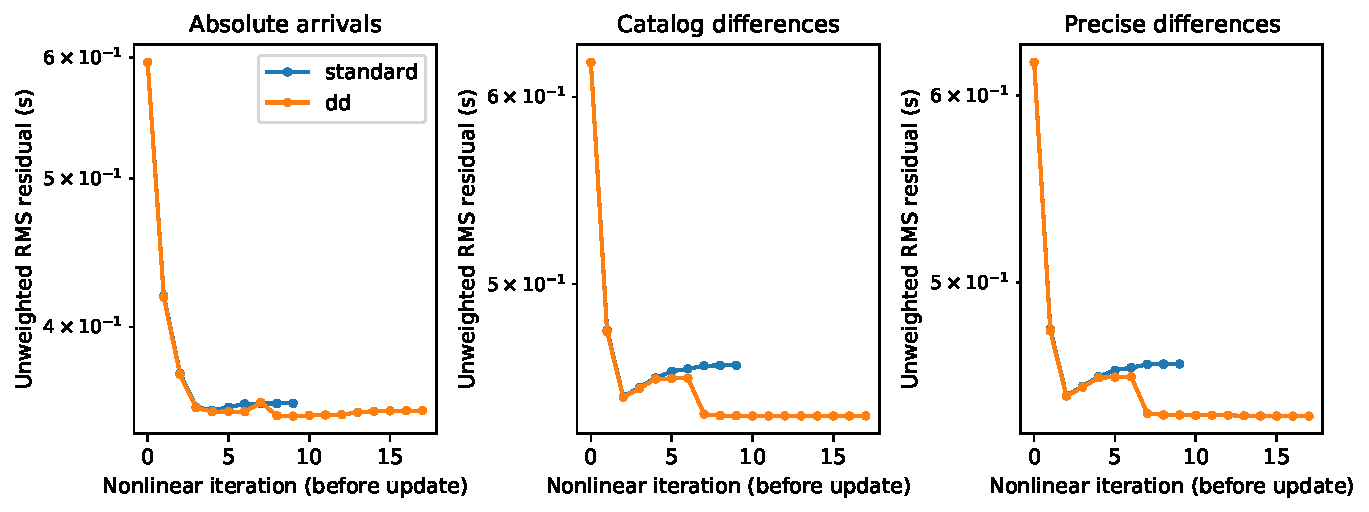
\includegraphics[width=\textwidth]{convergence.pdf}\\[1em]
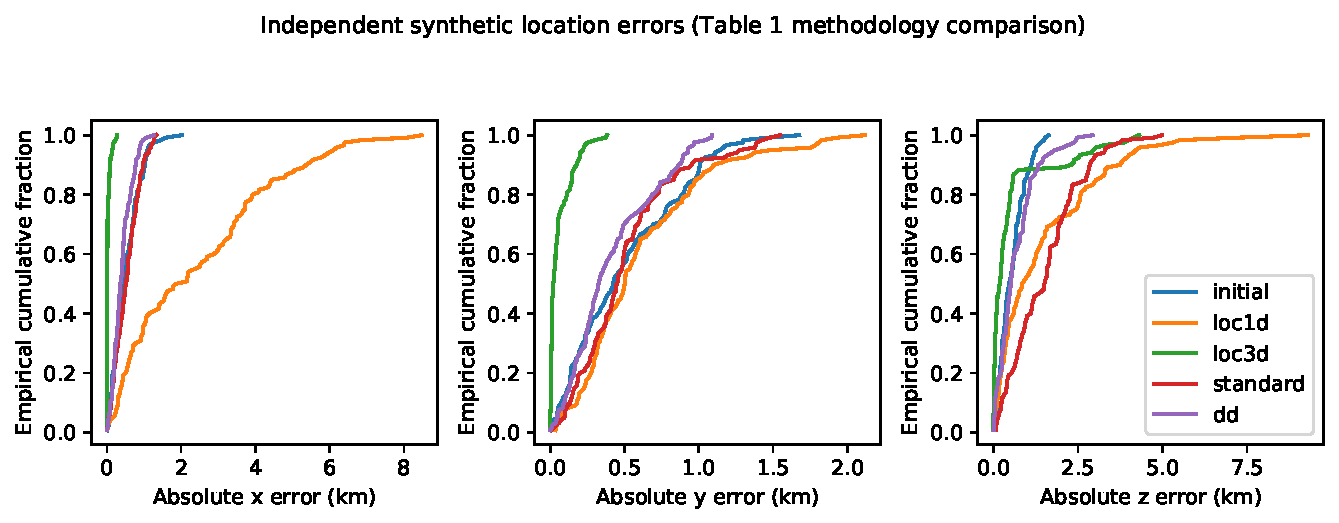
\includegraphics[width=\textwidth]{location_errors.pdf}
\caption{Independent convergence and location-error diagnostics. Top: RMS
residuals before each nonlinear update. Stage transitions change the objective,
so the unweighted RMS can rise while a weighted objective falls. Bottom:
source-coordinate error distributions against saved true coordinates.
These are additional method tests, not field-data panels.}
\end{figure}

\section{Discrepancies and reproduction limits}
The largest structural difference from the target experiment is its sampling
geometry. The synthetic coordinates in the original paper come from actual
seismicity and station locations, not from a distribution completely specified
in the text. Replacing that geometry changes the null space, ray coverage,
and source--velocity trade-off. A homogeneous initial velocity also changes
the nonlinear trajectory relative to the referenced layered model. We cannot
attribute a mismatch with a published error statistic solely to the inversion
algorithm under these changes.

Our forward grid represents the trough edges more finely than the inversion
grid. This is a deliberate test of model representation error. The 0.3 s
station biases are larger than the random pick errors, and the inverse
problem has no explicit station-static parameters. It must accommodate
these errors through source shifts, near-station velocity, or residual misfit.
Robust weighting may suppress genuine model mismatch as if it were an
outlier. A lower weighted objective therefore does not by itself establish
a more accurate velocity model; velocity and location errors against the
independent truth are reported separately.

During development, rejecting an entire trial update when one source left
the domain caused the fixed-model inversion to stall. Projecting individual
trial source locations onto the domain corrected that numerical obstruction.
Independent review also found that boundary directions within the ray
optimizer could block tangential motion, and that collapsed ray segments
could corrupt endpoint derivatives. Both cases now have numerical regression
checks. A further check found roundoff gradients in coordinate directions
where velocity was exactly constant. Ray optimization and column scaling
amplified these into spurious source-depth sensitivities. Evaluating each
interpolation-gradient component with paired nodal differences preserves
this symmetry exactly without changing the mathematical interpolant.
Constant-axis and surface-ray regression checks cover the correction.
The earlier numerical histories are retained in \path{data/development/}; they are
not used for any final numerical panel. Domain projection does not make
sources pinned to boundaries physically reliable.
In the depth-independent true medium, a source at the surface has zero
first-order depth sensitivity to the surface receivers. A linearized
fixed-model relocation therefore cannot move such a source back into the
interior. The boundary counts record this remaining geometric limitation;
the symmetry correction removes numerical drift rather than supplying
missing depth sensitivity.

For Hayward Figures 4--11, the missing dependencies are observational.
The field velocity model is the result to be inferred, not an input that can
be reconstructed by assuming the reported contrast. We recovered the written
grid, projection conventions, sample counts and section definitions, then
traced each panel's required data. These attempts stop at excluded arrivals
and event coordinates. In particular, resolution and uncertainty require
the actual linearized ray matrix, damping convention and covariance model.
A synthetic resolution matrix would not reproduce Figure 11, so none is
substituted here.

\section{Rebuild and artifact provenance}
Run the following command from the project root:
\begin{lstlisting}
./rebuild.sh
\end{lstlisting}
It configures and builds C++, runs validation, generates observations,
performs four main inversion comparisons, two starting-profile sensitivities,
fixed-model and joint recovery tests, and true/final-model ray checks,
computes metrics,
generates all figures and audit tables, and compiles this report twice with
pdfLaTeX. Its outcome is recorded in \path{data/rebuild_result.txt} only
when all commands have succeeded. Machine-readable numerical checks and
iteration histories remain in \path{data/}; raw console logs are local
diagnostics excluded from the shared repository. All caches and build intermediates
are confined to the project directory.

For this delivery, the complete clean procedure finished successfully on
9 October 2026 in 801 seconds, with all 32 implementation consistency checks
passing and both PDF compilation passes completing. The numerical results
come from that run. \path{reference/delivery_environment.json} records the
compiler, Python packages, TeX version, and parallel settings.
The final interpretation and plot-label revisions were compiled afterward
from the same numerical outputs; no model inputs or inversion code changed.

Requirements are a C++17 compiler, CMake, OpenMP, Python with NumPy and
Matplotlib, and pdfLaTeX with standard packages. No tomography, optimization,
or authors' software dependency is required. The saved input CSV files
permit rerunning the inverse problem without regenerating random numbers.
Standard-library random distributions may differ across platforms, so
cross-platform bitwise equality of newly generated observations is not
assumed. The experiment configuration, source code, plotting scripts,
generated data and figure audit are retained with this LaTeX source.

\clearpage
\appendix
\section{Numerical validation record}\label{sec:validation}
\begin{longtable}{lrr}\toprule Check & Error & Tolerance\\\midrule
homogeneous\_travel\_time & 4.44e-15 & 1e-10\\
homogeneous\_source\_derivative & 5.19e-17 & 1e-09\\
homogeneous\_velocity\_derivative & 4.44e-16 & 1e-09\\
partition\_of\_unity & 1.42e-14 & 1e-09\\
ray\_reciprocity & 6.58e-07 & 2e-05\\
bending\_not\_slower\_than\_straight & 0 & 1e-10\\
ray\_refinement\_seconds & 4.14e-05 & 0.015\\
bent\_source\_finite\_difference & 9.22e-05 & 0.003\\
velocity\_finite\_difference & 3.71e-13 & 1e-07\\
identical\_event\_dd\_cancellation & 0 & 1e-12\\
station\_bias\_cancellation & 0 & 1e-12\\
lsqr\_known\_solution & 7.11e-16 & 1e-09\\
matrix\_adjoint & 0 & 1e-12\\
interpolation\_constant\_x\_symmetry & 0 & 0\\
interpolation\_constant\_y\_symmetry & 0 & 0\\
interpolation\_constant\_z\_symmetry & 0 & 0\\
surface\_ray\_plane\_symmetry & 0 & 0\\
surface\_ray\_source\_symmetry & 0 & 0\\
snell\_reference\_travel\_time & 6.9e-05 & 0.001\\
snell\_reference\_source\_derivative & 8e-06 & 0.0001\\
trilinear\_gradient\_finite\_difference & 3.52e-12 & 2e-10\\
boundary\_ray\_feasible\_descent & 0 & 1e-10\\
boundary\_ray\_projected\_gradient & 1.84e-06 & 1e-05\\
boundary\_ray\_domain & 0 & 0\\
collapsed\_vertices\_preserve\_endpoints & 0 & 0\\
collapsed\_ray\_minimum\_segment & 0 & 0\\
collapsed\_ray\_gradient\_regression & 4.53e-05 & 0.001\\
scaled\_damped\_lsqr\_solution & 2.48e-16 & 1e-10\\
scaled\_damped\_lsqr\_normal\_residual & 5.55e-17 & 1e-08\\
scaled\_damped\_lsqr\_converged & 0 & 0\\
zero\_rhs\_lsqr & 0 & 0\\
truncated\_lsqr\_not\_converged & 0 & 0\\
\bottomrule\end{longtable}

Error units follow each test: seconds for time comparisons, seconds per km
for source derivatives, seconds per (km/s) for velocity derivatives, and
algebraic units for the sparse-system checks. These tolerances were chosen
for numerical consistency tests, not to enforce agreement with the paper.

\section{Figure-by-figure record}
The complete machine-readable record is in \path{data/panel_audit.csv}
and \path{data/panel_audit.json}; its readable counterpart is
\path{FIGURE_AUDIT.md}. ``Independently reproduced'' means the quantity is
reconstructed from the written specification using our model output.
``Partially reproduced'' means an independent numerical counterpart exists
but one or more specified experimental inputs or algorithms differ.
``Not reproduced'' means no corresponding result is claimed.
\begin{longtable}{p{0.13\textwidth}p{0.28\textwidth}p{0.48\textwidth}}\toprule Panel & Quantity & Status and limiting dependency\\\midrule\endhead
1 & Horizontal true P-velocity slice & independently reproduced. Physical velocity profile reconstructed from prose; plotting extent and depth chosen from model domain.\\
2 & Synthetic-test event/station geometry and inversion grid & partially reproduced. Grid recovered from caption. Original Loma Prieta coordinates are excluded and are not reconstructed from map pixels.\\
3a & Standard tomographic P velocity; all generated depth slices & partially reproduced. Independent geometry, homogeneous initial velocity, and explicit replacements for unpublished numerical settings; numerical comparisons cannot isolate implementation from experiment differences.\\
3b & DD tomographic P velocity; all generated depth slices & partially reproduced. Independent geometry, homogeneous initial velocity, and explicit replacements for unpublished numerical settings; numerical comparisons cannot isolate implementation from experiment differences.\\
3c & True minus DD P velocity; all generated depth slices & partially reproduced. Independent geometry, homogeneous initial velocity, and explicit replacements for unpublished numerical settings; numerical comparisons cannot isolate implementation from experiment differences.\\
3d & True minus standard P velocity; all generated depth slices & partially reproduced. Independent geometry, homogeneous initial velocity, and explicit replacements for unpublished numerical settings; numerical comparisons cannot isolate implementation from experiment differences.\\
4 & Hayward network, catalog seismicity, and inversion grid & not reproduced. Attempt: recovered written grid and required observation counts; no authorized coordinates for 1489 events or 52 stations. No invented field map is presented.\\
5a & Hayward event map: NCSN catalog & not reproduced. Attempt: traced input dependencies. Catalog picks, differential times and event identities cannot be inferred from written descriptions or regenerated by a physical forward model.\\
5b & Hayward event map: standard tomography & not reproduced. Attempt: traced input dependencies. Catalog picks, differential times and event identities cannot be inferred from written descriptions or regenerated by a physical forward model.\\
5c & Hayward event map: DD location & not reproduced. Attempt: traced input dependencies. Catalog picks, differential times and event identities cannot be inferred from written descriptions or regenerated by a physical forward model.\\
5d & Hayward event map: DD tomography & not reproduced. Attempt: traced input dependencies. Catalog picks, differential times and event identities cannot be inferred from written descriptions or regenerated by a physical forward model.\\
6a & catalog: geographical map & not reproduced. Attempt: recovered projection convention and regional selection. Input event locations/identities and, for c/d, box membership are unavailable under the data restriction. No digitization used.\\
6b & catalog: rotated Cartesian map & not reproduced. Attempt: recovered projection convention and regional selection. Input event locations/identities and, for c/d, box membership are unavailable under the data restriction. No digitization used.\\
6c & catalog: across-strike depth section AA-prime & not reproduced. Attempt: recovered projection convention and regional selection. Input event locations/identities and, for c/d, box membership are unavailable under the data restriction. No digitization used.\\
6d & catalog: along-strike depth section BB-prime & not reproduced. Attempt: recovered projection convention and regional selection. Input event locations/identities and, for c/d, box membership are unavailable under the data restriction. No digitization used.\\
7a & standard tomography: geographical map & not reproduced. Attempt: recovered projection convention and regional selection. Input event locations/identities and, for c/d, box membership are unavailable under the data restriction. No digitization used.\\
7b & standard tomography: rotated Cartesian map & not reproduced. Attempt: recovered projection convention and regional selection. Input event locations/identities and, for c/d, box membership are unavailable under the data restriction. No digitization used.\\
7c & standard tomography: across-strike depth section AA-prime & not reproduced. Attempt: recovered projection convention and regional selection. Input event locations/identities and, for c/d, box membership are unavailable under the data restriction. No digitization used.\\
7d & standard tomography: along-strike depth section BB-prime & not reproduced. Attempt: recovered projection convention and regional selection. Input event locations/identities and, for c/d, box membership are unavailable under the data restriction. No digitization used.\\
8a & DD location: geographical map & not reproduced. Attempt: recovered projection convention and regional selection. Input event locations/identities and, for c/d, box membership are unavailable under the data restriction. No digitization used.\\
8b & DD location: rotated Cartesian map & not reproduced. Attempt: recovered projection convention and regional selection. Input event locations/identities and, for c/d, box membership are unavailable under the data restriction. No digitization used.\\
8c & DD location: across-strike depth section AA-prime & not reproduced. Attempt: recovered projection convention and regional selection. Input event locations/identities and, for c/d, box membership are unavailable under the data restriction. No digitization used.\\
8d & DD location: along-strike depth section BB-prime & not reproduced. Attempt: recovered projection convention and regional selection. Input event locations/identities and, for c/d, box membership are unavailable under the data restriction. No digitization used.\\
9a & DD tomography: geographical map & not reproduced. Attempt: recovered projection convention and regional selection. Input event locations/identities and, for c/d, box membership are unavailable under the data restriction. No digitization used.\\
9b & DD tomography: rotated Cartesian map & not reproduced. Attempt: recovered projection convention and regional selection. Input event locations/identities and, for c/d, box membership are unavailable under the data restriction. No digitization used.\\
9c & DD tomography: across-strike depth section AA-prime & not reproduced. Attempt: recovered projection convention and regional selection. Input event locations/identities and, for c/d, box membership are unavailable under the data restriction. No digitization used.\\
9d & DD tomography: along-strike depth section BB-prime & not reproduced. Attempt: recovered projection convention and regional selection. Input event locations/identities and, for c/d, box membership are unavailable under the data restriction. No digitization used.\\
10a (y=-30) & Hayward across-strike DD velocity & not reproduced. Attempt: recovered grid, smoothing choice and cross-section convention. The observational velocity contrast is an inversion result, not a forward-model input specified by prose.\\
10a (y=-20) & Hayward across-strike DD velocity & not reproduced. Attempt: recovered grid, smoothing choice and cross-section convention. The observational velocity contrast is an inversion result, not a forward-model input specified by prose.\\
10a (y=-10) & Hayward across-strike DD velocity & not reproduced. Attempt: recovered grid, smoothing choice and cross-section convention. The observational velocity contrast is an inversion result, not a forward-model input specified by prose.\\
10a (y=0) & Hayward across-strike DD velocity & not reproduced. Attempt: recovered grid, smoothing choice and cross-section convention. The observational velocity contrast is an inversion result, not a forward-model input specified by prose.\\
10a (y=10) & Hayward across-strike DD velocity & not reproduced. Attempt: recovered grid, smoothing choice and cross-section convention. The observational velocity contrast is an inversion result, not a forward-model input specified by prose.\\
10a (y=20) & Hayward across-strike DD velocity & not reproduced. Attempt: recovered grid, smoothing choice and cross-section convention. The observational velocity contrast is an inversion result, not a forward-model input specified by prose.\\
10a (y=30) & Hayward across-strike DD velocity & not reproduced. Attempt: recovered grid, smoothing choice and cross-section convention. The observational velocity contrast is an inversion result, not a forward-model input specified by prose.\\
10b (y=-30) & Hayward across-strike standard velocity & not reproduced. Attempt: recovered grid, smoothing choice and cross-section convention. The observational velocity contrast is an inversion result, not a forward-model input specified by prose.\\
10b (y=-20) & Hayward across-strike standard velocity & not reproduced. Attempt: recovered grid, smoothing choice and cross-section convention. The observational velocity contrast is an inversion result, not a forward-model input specified by prose.\\
10b (y=-10) & Hayward across-strike standard velocity & not reproduced. Attempt: recovered grid, smoothing choice and cross-section convention. The observational velocity contrast is an inversion result, not a forward-model input specified by prose.\\
10b (y=0) & Hayward across-strike standard velocity & not reproduced. Attempt: recovered grid, smoothing choice and cross-section convention. The observational velocity contrast is an inversion result, not a forward-model input specified by prose.\\
10b (y=10) & Hayward across-strike standard velocity & not reproduced. Attempt: recovered grid, smoothing choice and cross-section convention. The observational velocity contrast is an inversion result, not a forward-model input specified by prose.\\
10b (y=20) & Hayward across-strike standard velocity & not reproduced. Attempt: recovered grid, smoothing choice and cross-section convention. The observational velocity contrast is an inversion result, not a forward-model input specified by prose.\\
10b (y=30) & Hayward across-strike standard velocity & not reproduced. Attempt: recovered grid, smoothing choice and cross-section convention. The observational velocity contrast is an inversion result, not a forward-model input specified by prose.\\
10c (y=-30) & Hayward across-strike DD minus standard velocity & not reproduced. Attempt: recovered grid, smoothing choice and cross-section convention. The observational velocity contrast is an inversion result, not a forward-model input specified by prose.\\
10c (y=-20) & Hayward across-strike DD minus standard velocity & not reproduced. Attempt: recovered grid, smoothing choice and cross-section convention. The observational velocity contrast is an inversion result, not a forward-model input specified by prose.\\
10c (y=-10) & Hayward across-strike DD minus standard velocity & not reproduced. Attempt: recovered grid, smoothing choice and cross-section convention. The observational velocity contrast is an inversion result, not a forward-model input specified by prose.\\
10c (y=0) & Hayward across-strike DD minus standard velocity & not reproduced. Attempt: recovered grid, smoothing choice and cross-section convention. The observational velocity contrast is an inversion result, not a forward-model input specified by prose.\\
10c (y=10) & Hayward across-strike DD minus standard velocity & not reproduced. Attempt: recovered grid, smoothing choice and cross-section convention. The observational velocity contrast is an inversion result, not a forward-model input specified by prose.\\
10c (y=20) & Hayward across-strike DD minus standard velocity & not reproduced. Attempt: recovered grid, smoothing choice and cross-section convention. The observational velocity contrast is an inversion result, not a forward-model input specified by prose.\\
10c (y=30) & Hayward across-strike DD minus standard velocity & not reproduced. Attempt: recovered grid, smoothing choice and cross-section convention. The observational velocity contrast is an inversion result, not a forward-model input specified by prose.\\
11a (y=-30) & Hayward resolution-matrix diagonal & not reproduced. Attempt: established dependency on the actual ray geometry, final field model, damping and data covariance. These cannot be replaced by an unrelated synthetic resolution matrix and called a reproduction.\\
11a (y=-20) & Hayward resolution-matrix diagonal & not reproduced. Attempt: established dependency on the actual ray geometry, final field model, damping and data covariance. These cannot be replaced by an unrelated synthetic resolution matrix and called a reproduction.\\
11a (y=-10) & Hayward resolution-matrix diagonal & not reproduced. Attempt: established dependency on the actual ray geometry, final field model, damping and data covariance. These cannot be replaced by an unrelated synthetic resolution matrix and called a reproduction.\\
11a (y=0) & Hayward resolution-matrix diagonal & not reproduced. Attempt: established dependency on the actual ray geometry, final field model, damping and data covariance. These cannot be replaced by an unrelated synthetic resolution matrix and called a reproduction.\\
11a (y=10) & Hayward resolution-matrix diagonal & not reproduced. Attempt: established dependency on the actual ray geometry, final field model, damping and data covariance. These cannot be replaced by an unrelated synthetic resolution matrix and called a reproduction.\\
11a (y=20) & Hayward resolution-matrix diagonal & not reproduced. Attempt: established dependency on the actual ray geometry, final field model, damping and data covariance. These cannot be replaced by an unrelated synthetic resolution matrix and called a reproduction.\\
11a (y=30) & Hayward resolution-matrix diagonal & not reproduced. Attempt: established dependency on the actual ray geometry, final field model, damping and data covariance. These cannot be replaced by an unrelated synthetic resolution matrix and called a reproduction.\\
11b (y=-30) & Hayward one-sigma velocity uncertainty & not reproduced. Attempt: established dependency on the actual ray geometry, final field model, damping and data covariance. These cannot be replaced by an unrelated synthetic resolution matrix and called a reproduction.\\
11b (y=-20) & Hayward one-sigma velocity uncertainty & not reproduced. Attempt: established dependency on the actual ray geometry, final field model, damping and data covariance. These cannot be replaced by an unrelated synthetic resolution matrix and called a reproduction.\\
11b (y=-10) & Hayward one-sigma velocity uncertainty & not reproduced. Attempt: established dependency on the actual ray geometry, final field model, damping and data covariance. These cannot be replaced by an unrelated synthetic resolution matrix and called a reproduction.\\
11b (y=0) & Hayward one-sigma velocity uncertainty & not reproduced. Attempt: established dependency on the actual ray geometry, final field model, damping and data covariance. These cannot be replaced by an unrelated synthetic resolution matrix and called a reproduction.\\
11b (y=10) & Hayward one-sigma velocity uncertainty & not reproduced. Attempt: established dependency on the actual ray geometry, final field model, damping and data covariance. These cannot be replaced by an unrelated synthetic resolution matrix and called a reproduction.\\
11b (y=20) & Hayward one-sigma velocity uncertainty & not reproduced. Attempt: established dependency on the actual ray geometry, final field model, damping and data covariance. These cannot be replaced by an unrelated synthetic resolution matrix and called a reproduction.\\
11b (y=30) & Hayward one-sigma velocity uncertainty & not reproduced. Attempt: established dependency on the actual ray geometry, final field model, damping and data covariance. These cannot be replaced by an unrelated synthetic resolution matrix and called a reproduction.\\
\bottomrule\end{longtable}

\subsection{Specifications, commands, and attempted dependencies}
The following records specify the source description, parameters, generation
command, and plot command for each panel. Seven sections of a common
Figure 10 or 11 panel share the explicitly listed settings. Unavailable
commands are reported as unavailable rather than replaced by placeholders
that would fabricate field observations.
\subsubsection*{Panel 1}
\noindent\textbf{Quantity:} Horizontal true P-velocity slice\par
\noindent\textbf{Written specification:} Synthetic Test, p.1877; caption 1\par
\noindent\textbf{Parameters:} Written sandwich profile, x=-35..35 km, y=-60..40 km; constant with depth\par
\noindent\textbf{Status:} independently reproduced\par
\noindent\textbf{Attempt and limitation:} Physical velocity profile reconstructed from prose; plotting extent and depth chosen from model domain.\par
\noindent\textbf{Generate data:}
\begin{lstlisting}
./build/dd generate configs/synthetic.cfg data/synthetic
\end{lstlisting}
\noindent\textbf{Create plot:}
\begin{lstlisting}
python3 plot.py --figure 1
\end{lstlisting}
\subsubsection*{Panel 2}
\noindent\textbf{Quantity:} Synthetic-test event/station geometry and inversion grid\par
\noindent\textbf{Written specification:} Caption 2, p.1879\par
\noindent\textbf{Parameters:} Published 8x6x5 inversion grid; 120 independent sources and 32 independent stations, seed 2003\par
\noindent\textbf{Status:} partially reproduced\par
\noindent\textbf{Attempt and limitation:} Grid recovered from caption. Original Loma Prieta coordinates are excluded and are not reconstructed from map pixels.\par
\noindent\textbf{Generate data:}
\begin{lstlisting}
./build/dd generate configs/synthetic.cfg data/synthetic
\end{lstlisting}
\noindent\textbf{Create plot:}
\begin{lstlisting}
python3 plot.py --figure 2
\end{lstlisting}
\subsubsection*{Panel 3a}
\noindent\textbf{Quantity:} Standard tomographic P velocity; all generated depth slices\par
\noindent\textbf{Written specification:} Synthetic Test pp.1877-1879; captions 3 pp.1880-1881\par
\noindent\textbf{Parameters:} Depths 0,3,7,11,16 km; grid from caption 2; noise 0.04 s and station bias +/-0.3 s; configs/synthetic.cfg\par
\noindent\textbf{Status:} partially reproduced\par
\noindent\textbf{Attempt and limitation:} Independent geometry, homogeneous initial velocity, and explicit replacements for unpublished numerical settings; numerical comparisons cannot isolate implementation from experiment differences.\par
\noindent\textbf{Generate data:}
\begin{lstlisting}
./build/dd generate configs/synthetic.cfg data/synthetic && ./build/dd invert configs/synthetic.cfg data/synthetic standard
\end{lstlisting}
\noindent\textbf{Create plot:}
\begin{lstlisting}
python3 plot.py --figure 3a
\end{lstlisting}
\subsubsection*{Panel 3b}
\noindent\textbf{Quantity:} DD tomographic P velocity; all generated depth slices\par
\noindent\textbf{Written specification:} Synthetic Test pp.1877-1879; captions 3 pp.1880-1881\par
\noindent\textbf{Parameters:} Depths 0,3,7,11,16 km; grid from caption 2; noise 0.04 s and station bias +/-0.3 s; configs/synthetic.cfg\par
\noindent\textbf{Status:} partially reproduced\par
\noindent\textbf{Attempt and limitation:} Independent geometry, homogeneous initial velocity, and explicit replacements for unpublished numerical settings; numerical comparisons cannot isolate implementation from experiment differences.\par
\noindent\textbf{Generate data:}
\begin{lstlisting}
./build/dd generate configs/synthetic.cfg data/synthetic && ./build/dd invert configs/synthetic.cfg data/synthetic dd
\end{lstlisting}
\noindent\textbf{Create plot:}
\begin{lstlisting}
python3 plot.py --figure 3b
\end{lstlisting}
\subsubsection*{Panel 3c}
\noindent\textbf{Quantity:} True minus DD P velocity; all generated depth slices\par
\noindent\textbf{Written specification:} Synthetic Test pp.1877-1879; captions 3 pp.1880-1881\par
\noindent\textbf{Parameters:} Depths 0,3,7,11,16 km; grid from caption 2; noise 0.04 s and station bias +/-0.3 s; configs/synthetic.cfg\par
\noindent\textbf{Status:} partially reproduced\par
\noindent\textbf{Attempt and limitation:} Independent geometry, homogeneous initial velocity, and explicit replacements for unpublished numerical settings; numerical comparisons cannot isolate implementation from experiment differences.\par
\noindent\textbf{Generate data:}
\begin{lstlisting}
./build/dd generate configs/synthetic.cfg data/synthetic && ./build/dd invert configs/synthetic.cfg data/synthetic dd
\end{lstlisting}
\noindent\textbf{Create plot:}
\begin{lstlisting}
python3 plot.py --figure 3c
\end{lstlisting}
\subsubsection*{Panel 3d}
\noindent\textbf{Quantity:} True minus standard P velocity; all generated depth slices\par
\noindent\textbf{Written specification:} Synthetic Test pp.1877-1879; captions 3 pp.1880-1881\par
\noindent\textbf{Parameters:} Depths 0,3,7,11,16 km; grid from caption 2; noise 0.04 s and station bias +/-0.3 s; configs/synthetic.cfg\par
\noindent\textbf{Status:} partially reproduced\par
\noindent\textbf{Attempt and limitation:} Independent geometry, homogeneous initial velocity, and explicit replacements for unpublished numerical settings; numerical comparisons cannot isolate implementation from experiment differences.\par
\noindent\textbf{Generate data:}
\begin{lstlisting}
./build/dd generate configs/synthetic.cfg data/synthetic && ./build/dd invert configs/synthetic.cfg data/synthetic standard
\end{lstlisting}
\noindent\textbf{Create plot:}
\begin{lstlisting}
python3 plot.py --figure 3d
\end{lstlisting}
\subsubsection*{Panel 4}
\noindent\textbf{Quantity:} Hayward network, catalog seismicity, and inversion grid\par
\noindent\textbf{Written specification:} Caption 4, p.1882\par
\noindent\textbf{Parameters:} Grid x=-35,-20,-10,-5,-4,-3,0,5,10,20,35; y=-30,-20,-10,0,10,20,30; z=0,4,8,12,20 km\par
\noindent\textbf{Status:} not reproduced\par
\noindent\textbf{Attempt and limitation:} Attempt: recovered written grid and required observation counts; no authorized coordinates for 1489 events or 52 stations. No invented field map is presented.\par
\noindent\textbf{Generate data:}
\begin{lstlisting}
Unavailable: requires excluded observed coordinates
\end{lstlisting}
\noindent\textbf{Create plot:}
\begin{lstlisting}
Unavailable: no source data
\end{lstlisting}
\subsubsection*{Panel 5a}
\noindent\textbf{Quantity:} Hayward event map: NCSN catalog\par
\noindent\textbf{Written specification:} Event Locations pp.1881-1883; caption 5\par
\noindent\textbf{Parameters:} 1489 earthquakes, 52 stations; 20257 absolute picks, 767127 catalog differences, 17955 precise differences\par
\noindent\textbf{Status:} not reproduced\par
\noindent\textbf{Attempt and limitation:} Attempt: traced input dependencies. Catalog picks, differential times and event identities cannot be inferred from written descriptions or regenerated by a physical forward model.\par
\noindent\textbf{Generate data:}
\begin{lstlisting}
Unavailable: requires excluded observations
\end{lstlisting}
\noindent\textbf{Create plot:}
\begin{lstlisting}
Unavailable: no source data
\end{lstlisting}
\subsubsection*{Panel 5b}
\noindent\textbf{Quantity:} Hayward event map: standard tomography\par
\noindent\textbf{Written specification:} Event Locations pp.1881-1883; caption 5\par
\noindent\textbf{Parameters:} 1489 earthquakes, 52 stations; 20257 absolute picks, 767127 catalog differences, 17955 precise differences\par
\noindent\textbf{Status:} not reproduced\par
\noindent\textbf{Attempt and limitation:} Attempt: traced input dependencies. Catalog picks, differential times and event identities cannot be inferred from written descriptions or regenerated by a physical forward model.\par
\noindent\textbf{Generate data:}
\begin{lstlisting}
Unavailable: requires excluded observations
\end{lstlisting}
\noindent\textbf{Create plot:}
\begin{lstlisting}
Unavailable: no source data
\end{lstlisting}
\subsubsection*{Panel 5c}
\noindent\textbf{Quantity:} Hayward event map: DD location\par
\noindent\textbf{Written specification:} Event Locations pp.1881-1883; caption 5\par
\noindent\textbf{Parameters:} 1489 earthquakes, 52 stations; 20257 absolute picks, 767127 catalog differences, 17955 precise differences\par
\noindent\textbf{Status:} not reproduced\par
\noindent\textbf{Attempt and limitation:} Attempt: traced input dependencies. Catalog picks, differential times and event identities cannot be inferred from written descriptions or regenerated by a physical forward model.\par
\noindent\textbf{Generate data:}
\begin{lstlisting}
Unavailable: requires excluded observations
\end{lstlisting}
\noindent\textbf{Create plot:}
\begin{lstlisting}
Unavailable: no source data
\end{lstlisting}
\subsubsection*{Panel 5d}
\noindent\textbf{Quantity:} Hayward event map: DD tomography\par
\noindent\textbf{Written specification:} Event Locations pp.1881-1883; caption 5\par
\noindent\textbf{Parameters:} 1489 earthquakes, 52 stations; 20257 absolute picks, 767127 catalog differences, 17955 precise differences\par
\noindent\textbf{Status:} not reproduced\par
\noindent\textbf{Attempt and limitation:} Attempt: traced input dependencies. Catalog picks, differential times and event identities cannot be inferred from written descriptions or regenerated by a physical forward model.\par
\noindent\textbf{Generate data:}
\begin{lstlisting}
Unavailable: requires excluded observations
\end{lstlisting}
\noindent\textbf{Create plot:}
\begin{lstlisting}
Unavailable: no source data
\end{lstlisting}
\subsubsection*{Panel 6a}
\noindent\textbf{Quantity:} catalog: geographical map\par
\noindent\textbf{Written specification:} Event Locations pp.1882-1884; captions 6-9\par
\noindent\textbf{Parameters:} Center 37.72 N, 122.06 W; 35-degree anticlockwise rotation; map selection 37.83..37.91 N, -122.26..-122.18 E\par
\noindent\textbf{Status:} not reproduced\par
\noindent\textbf{Attempt and limitation:} Attempt: recovered projection convention and regional selection. Input event locations/identities and, for c/d, box membership are unavailable under the data restriction. No digitization used.\par
\noindent\textbf{Generate data:}
\begin{lstlisting}
Unavailable: requires excluded event catalog and travel times
\end{lstlisting}
\noindent\textbf{Create plot:}
\begin{lstlisting}
Unavailable: no source data
\end{lstlisting}
\subsubsection*{Panel 6b}
\noindent\textbf{Quantity:} catalog: rotated Cartesian map\par
\noindent\textbf{Written specification:} Event Locations pp.1882-1884; captions 6-9\par
\noindent\textbf{Parameters:} Center 37.72 N, 122.06 W; 35-degree anticlockwise rotation; map selection 37.83..37.91 N, -122.26..-122.18 E\par
\noindent\textbf{Status:} not reproduced\par
\noindent\textbf{Attempt and limitation:} Attempt: recovered projection convention and regional selection. Input event locations/identities and, for c/d, box membership are unavailable under the data restriction. No digitization used.\par
\noindent\textbf{Generate data:}
\begin{lstlisting}
Unavailable: requires excluded event catalog and travel times
\end{lstlisting}
\noindent\textbf{Create plot:}
\begin{lstlisting}
Unavailable: no source data
\end{lstlisting}
\subsubsection*{Panel 6c}
\noindent\textbf{Quantity:} catalog: across-strike depth section AA-prime\par
\noindent\textbf{Written specification:} Event Locations pp.1882-1884; captions 6-9\par
\noindent\textbf{Parameters:} Center 37.72 N, 122.06 W; 35-degree anticlockwise rotation; map selection 37.83..37.91 N, -122.26..-122.18 E\par
\noindent\textbf{Status:} not reproduced\par
\noindent\textbf{Attempt and limitation:} Attempt: recovered projection convention and regional selection. Input event locations/identities and, for c/d, box membership are unavailable under the data restriction. No digitization used.\par
\noindent\textbf{Generate data:}
\begin{lstlisting}
Unavailable: requires excluded event catalog and travel times
\end{lstlisting}
\noindent\textbf{Create plot:}
\begin{lstlisting}
Unavailable: no source data
\end{lstlisting}
\subsubsection*{Panel 6d}
\noindent\textbf{Quantity:} catalog: along-strike depth section BB-prime\par
\noindent\textbf{Written specification:} Event Locations pp.1882-1884; captions 6-9\par
\noindent\textbf{Parameters:} Center 37.72 N, 122.06 W; 35-degree anticlockwise rotation; map selection 37.83..37.91 N, -122.26..-122.18 E\par
\noindent\textbf{Status:} not reproduced\par
\noindent\textbf{Attempt and limitation:} Attempt: recovered projection convention and regional selection. Input event locations/identities and, for c/d, box membership are unavailable under the data restriction. No digitization used.\par
\noindent\textbf{Generate data:}
\begin{lstlisting}
Unavailable: requires excluded event catalog and travel times
\end{lstlisting}
\noindent\textbf{Create plot:}
\begin{lstlisting}
Unavailable: no source data
\end{lstlisting}
\subsubsection*{Panel 7a}
\noindent\textbf{Quantity:} standard tomography: geographical map\par
\noindent\textbf{Written specification:} Event Locations pp.1882-1884; captions 6-9\par
\noindent\textbf{Parameters:} Center 37.72 N, 122.06 W; 35-degree anticlockwise rotation; map selection 37.83..37.91 N, -122.26..-122.18 E\par
\noindent\textbf{Status:} not reproduced\par
\noindent\textbf{Attempt and limitation:} Attempt: recovered projection convention and regional selection. Input event locations/identities and, for c/d, box membership are unavailable under the data restriction. No digitization used.\par
\noindent\textbf{Generate data:}
\begin{lstlisting}
Unavailable: requires excluded event catalog and travel times
\end{lstlisting}
\noindent\textbf{Create plot:}
\begin{lstlisting}
Unavailable: no source data
\end{lstlisting}
\subsubsection*{Panel 7b}
\noindent\textbf{Quantity:} standard tomography: rotated Cartesian map\par
\noindent\textbf{Written specification:} Event Locations pp.1882-1884; captions 6-9\par
\noindent\textbf{Parameters:} Center 37.72 N, 122.06 W; 35-degree anticlockwise rotation; map selection 37.83..37.91 N, -122.26..-122.18 E\par
\noindent\textbf{Status:} not reproduced\par
\noindent\textbf{Attempt and limitation:} Attempt: recovered projection convention and regional selection. Input event locations/identities and, for c/d, box membership are unavailable under the data restriction. No digitization used.\par
\noindent\textbf{Generate data:}
\begin{lstlisting}
Unavailable: requires excluded event catalog and travel times
\end{lstlisting}
\noindent\textbf{Create plot:}
\begin{lstlisting}
Unavailable: no source data
\end{lstlisting}
\subsubsection*{Panel 7c}
\noindent\textbf{Quantity:} standard tomography: across-strike depth section AA-prime\par
\noindent\textbf{Written specification:} Event Locations pp.1882-1884; captions 6-9\par
\noindent\textbf{Parameters:} Center 37.72 N, 122.06 W; 35-degree anticlockwise rotation; map selection 37.83..37.91 N, -122.26..-122.18 E\par
\noindent\textbf{Status:} not reproduced\par
\noindent\textbf{Attempt and limitation:} Attempt: recovered projection convention and regional selection. Input event locations/identities and, for c/d, box membership are unavailable under the data restriction. No digitization used.\par
\noindent\textbf{Generate data:}
\begin{lstlisting}
Unavailable: requires excluded event catalog and travel times
\end{lstlisting}
\noindent\textbf{Create plot:}
\begin{lstlisting}
Unavailable: no source data
\end{lstlisting}
\subsubsection*{Panel 7d}
\noindent\textbf{Quantity:} standard tomography: along-strike depth section BB-prime\par
\noindent\textbf{Written specification:} Event Locations pp.1882-1884; captions 6-9\par
\noindent\textbf{Parameters:} Center 37.72 N, 122.06 W; 35-degree anticlockwise rotation; map selection 37.83..37.91 N, -122.26..-122.18 E\par
\noindent\textbf{Status:} not reproduced\par
\noindent\textbf{Attempt and limitation:} Attempt: recovered projection convention and regional selection. Input event locations/identities and, for c/d, box membership are unavailable under the data restriction. No digitization used.\par
\noindent\textbf{Generate data:}
\begin{lstlisting}
Unavailable: requires excluded event catalog and travel times
\end{lstlisting}
\noindent\textbf{Create plot:}
\begin{lstlisting}
Unavailable: no source data
\end{lstlisting}
\subsubsection*{Panel 8a}
\noindent\textbf{Quantity:} DD location: geographical map\par
\noindent\textbf{Written specification:} Event Locations pp.1882-1884; captions 6-9\par
\noindent\textbf{Parameters:} Center 37.72 N, 122.06 W; 35-degree anticlockwise rotation; map selection 37.83..37.91 N, -122.26..-122.18 E\par
\noindent\textbf{Status:} not reproduced\par
\noindent\textbf{Attempt and limitation:} Attempt: recovered projection convention and regional selection. Input event locations/identities and, for c/d, box membership are unavailable under the data restriction. No digitization used.\par
\noindent\textbf{Generate data:}
\begin{lstlisting}
Unavailable: requires excluded event catalog and travel times
\end{lstlisting}
\noindent\textbf{Create plot:}
\begin{lstlisting}
Unavailable: no source data
\end{lstlisting}
\subsubsection*{Panel 8b}
\noindent\textbf{Quantity:} DD location: rotated Cartesian map\par
\noindent\textbf{Written specification:} Event Locations pp.1882-1884; captions 6-9\par
\noindent\textbf{Parameters:} Center 37.72 N, 122.06 W; 35-degree anticlockwise rotation; map selection 37.83..37.91 N, -122.26..-122.18 E\par
\noindent\textbf{Status:} not reproduced\par
\noindent\textbf{Attempt and limitation:} Attempt: recovered projection convention and regional selection. Input event locations/identities and, for c/d, box membership are unavailable under the data restriction. No digitization used.\par
\noindent\textbf{Generate data:}
\begin{lstlisting}
Unavailable: requires excluded event catalog and travel times
\end{lstlisting}
\noindent\textbf{Create plot:}
\begin{lstlisting}
Unavailable: no source data
\end{lstlisting}
\subsubsection*{Panel 8c}
\noindent\textbf{Quantity:} DD location: across-strike depth section AA-prime\par
\noindent\textbf{Written specification:} Event Locations pp.1882-1884; captions 6-9\par
\noindent\textbf{Parameters:} Center 37.72 N, 122.06 W; 35-degree anticlockwise rotation; map selection 37.83..37.91 N, -122.26..-122.18 E\par
\noindent\textbf{Status:} not reproduced\par
\noindent\textbf{Attempt and limitation:} Attempt: recovered projection convention and regional selection. Input event locations/identities and, for c/d, box membership are unavailable under the data restriction. No digitization used.\par
\noindent\textbf{Generate data:}
\begin{lstlisting}
Unavailable: requires excluded event catalog and travel times
\end{lstlisting}
\noindent\textbf{Create plot:}
\begin{lstlisting}
Unavailable: no source data
\end{lstlisting}
\subsubsection*{Panel 8d}
\noindent\textbf{Quantity:} DD location: along-strike depth section BB-prime\par
\noindent\textbf{Written specification:} Event Locations pp.1882-1884; captions 6-9\par
\noindent\textbf{Parameters:} Center 37.72 N, 122.06 W; 35-degree anticlockwise rotation; map selection 37.83..37.91 N, -122.26..-122.18 E\par
\noindent\textbf{Status:} not reproduced\par
\noindent\textbf{Attempt and limitation:} Attempt: recovered projection convention and regional selection. Input event locations/identities and, for c/d, box membership are unavailable under the data restriction. No digitization used.\par
\noindent\textbf{Generate data:}
\begin{lstlisting}
Unavailable: requires excluded event catalog and travel times
\end{lstlisting}
\noindent\textbf{Create plot:}
\begin{lstlisting}
Unavailable: no source data
\end{lstlisting}
\subsubsection*{Panel 9a}
\noindent\textbf{Quantity:} DD tomography: geographical map\par
\noindent\textbf{Written specification:} Event Locations pp.1882-1884; captions 6-9\par
\noindent\textbf{Parameters:} Center 37.72 N, 122.06 W; 35-degree anticlockwise rotation; map selection 37.83..37.91 N, -122.26..-122.18 E\par
\noindent\textbf{Status:} not reproduced\par
\noindent\textbf{Attempt and limitation:} Attempt: recovered projection convention and regional selection. Input event locations/identities and, for c/d, box membership are unavailable under the data restriction. No digitization used.\par
\noindent\textbf{Generate data:}
\begin{lstlisting}
Unavailable: requires excluded event catalog and travel times
\end{lstlisting}
\noindent\textbf{Create plot:}
\begin{lstlisting}
Unavailable: no source data
\end{lstlisting}
\subsubsection*{Panel 9b}
\noindent\textbf{Quantity:} DD tomography: rotated Cartesian map\par
\noindent\textbf{Written specification:} Event Locations pp.1882-1884; captions 6-9\par
\noindent\textbf{Parameters:} Center 37.72 N, 122.06 W; 35-degree anticlockwise rotation; map selection 37.83..37.91 N, -122.26..-122.18 E\par
\noindent\textbf{Status:} not reproduced\par
\noindent\textbf{Attempt and limitation:} Attempt: recovered projection convention and regional selection. Input event locations/identities and, for c/d, box membership are unavailable under the data restriction. No digitization used.\par
\noindent\textbf{Generate data:}
\begin{lstlisting}
Unavailable: requires excluded event catalog and travel times
\end{lstlisting}
\noindent\textbf{Create plot:}
\begin{lstlisting}
Unavailable: no source data
\end{lstlisting}
\subsubsection*{Panel 9c}
\noindent\textbf{Quantity:} DD tomography: across-strike depth section AA-prime\par
\noindent\textbf{Written specification:} Event Locations pp.1882-1884; captions 6-9\par
\noindent\textbf{Parameters:} Center 37.72 N, 122.06 W; 35-degree anticlockwise rotation; map selection 37.83..37.91 N, -122.26..-122.18 E\par
\noindent\textbf{Status:} not reproduced\par
\noindent\textbf{Attempt and limitation:} Attempt: recovered projection convention and regional selection. Input event locations/identities and, for c/d, box membership are unavailable under the data restriction. No digitization used.\par
\noindent\textbf{Generate data:}
\begin{lstlisting}
Unavailable: requires excluded event catalog and travel times
\end{lstlisting}
\noindent\textbf{Create plot:}
\begin{lstlisting}
Unavailable: no source data
\end{lstlisting}
\subsubsection*{Panel 9d}
\noindent\textbf{Quantity:} DD tomography: along-strike depth section BB-prime\par
\noindent\textbf{Written specification:} Event Locations pp.1882-1884; captions 6-9\par
\noindent\textbf{Parameters:} Center 37.72 N, 122.06 W; 35-degree anticlockwise rotation; map selection 37.83..37.91 N, -122.26..-122.18 E\par
\noindent\textbf{Status:} not reproduced\par
\noindent\textbf{Attempt and limitation:} Attempt: recovered projection convention and regional selection. Input event locations/identities and, for c/d, box membership are unavailable under the data restriction. No digitization used.\par
\noindent\textbf{Generate data:}
\begin{lstlisting}
Unavailable: requires excluded event catalog and travel times
\end{lstlisting}
\noindent\textbf{Create plot:}
\begin{lstlisting}
Unavailable: no source data
\end{lstlisting}
\subsubsection*{Panel 10a: all seven sections at y=-30,-20,-10,0,10,20,30 km}
\noindent\textbf{Quantity:} Hayward across-strike DD velocity\par
\noindent\textbf{Written specification:} Velocity Structure p.1884; caption 10 p.1887\par
\noindent\textbf{Parameters:} Published Hayward grid; smoothing weight 10; all seven y sections listed above; hypocenters within 5 km\par
\noindent\textbf{Status:} not reproduced\par
\noindent\textbf{Attempt and limitation:} Attempt: recovered grid, smoothing choice and cross-section convention. The observational velocity contrast is an inversion result, not a forward-model input specified by prose.\par
\noindent\textbf{Generate data:}
\begin{lstlisting}
Unavailable: requires excluded Hayward observations
\end{lstlisting}
\noindent\textbf{Create plot:}
\begin{lstlisting}
Unavailable: no field inversion output
\end{lstlisting}
\subsubsection*{Panel 10b: all seven sections at y=-30,-20,-10,0,10,20,30 km}
\noindent\textbf{Quantity:} Hayward across-strike standard velocity\par
\noindent\textbf{Written specification:} Velocity Structure p.1884; caption 10 p.1887\par
\noindent\textbf{Parameters:} Published Hayward grid; smoothing weight 10; all seven y sections listed above; hypocenters within 5 km\par
\noindent\textbf{Status:} not reproduced\par
\noindent\textbf{Attempt and limitation:} Attempt: recovered grid, smoothing choice and cross-section convention. The observational velocity contrast is an inversion result, not a forward-model input specified by prose.\par
\noindent\textbf{Generate data:}
\begin{lstlisting}
Unavailable: requires excluded Hayward observations
\end{lstlisting}
\noindent\textbf{Create plot:}
\begin{lstlisting}
Unavailable: no field inversion output
\end{lstlisting}
\subsubsection*{Panel 10c: all seven sections at y=-30,-20,-10,0,10,20,30 km}
\noindent\textbf{Quantity:} Hayward across-strike DD minus standard velocity\par
\noindent\textbf{Written specification:} Velocity Structure p.1884; caption 10 p.1887\par
\noindent\textbf{Parameters:} Published Hayward grid; smoothing weight 10; all seven y sections listed above; hypocenters within 5 km\par
\noindent\textbf{Status:} not reproduced\par
\noindent\textbf{Attempt and limitation:} Attempt: recovered grid, smoothing choice and cross-section convention. The observational velocity contrast is an inversion result, not a forward-model input specified by prose.\par
\noindent\textbf{Generate data:}
\begin{lstlisting}
Unavailable: requires excluded Hayward observations
\end{lstlisting}
\noindent\textbf{Create plot:}
\begin{lstlisting}
Unavailable: no field inversion output
\end{lstlisting}
\subsubsection*{Panel 11a: all seven sections at y=-30,-20,-10,0,10,20,30 km}
\noindent\textbf{Quantity:} Hayward resolution-matrix diagonal\par
\noindent\textbf{Written specification:} Velocity Structure pp.1884,1886; caption 11 p.1888\par
\noindent\textbf{Parameters:} Absolute-data standard-tomography linearization at the DD velocity model; all seven y sections listed above\par
\noindent\textbf{Status:} not reproduced\par
\noindent\textbf{Attempt and limitation:} Attempt: established dependency on the actual ray geometry, final field model, damping and data covariance. These cannot be replaced by an unrelated synthetic resolution matrix and called a reproduction.\par
\noindent\textbf{Generate data:}
\begin{lstlisting}
Unavailable: requires excluded observation matrix and inferred field velocity
\end{lstlisting}
\noindent\textbf{Create plot:}
\begin{lstlisting}
Unavailable: no field matrix
\end{lstlisting}
\subsubsection*{Panel 11b: all seven sections at y=-30,-20,-10,0,10,20,30 km}
\noindent\textbf{Quantity:} Hayward one-sigma velocity uncertainty\par
\noindent\textbf{Written specification:} Velocity Structure pp.1884,1886; caption 11 p.1888\par
\noindent\textbf{Parameters:} Absolute-data standard-tomography linearization at the DD velocity model; all seven y sections listed above\par
\noindent\textbf{Status:} not reproduced\par
\noindent\textbf{Attempt and limitation:} Attempt: established dependency on the actual ray geometry, final field model, damping and data covariance. These cannot be replaced by an unrelated synthetic resolution matrix and called a reproduction.\par
\noindent\textbf{Generate data:}
\begin{lstlisting}
Unavailable: requires excluded observation matrix and inferred field velocity
\end{lstlisting}
\noindent\textbf{Create plot:}
\begin{lstlisting}
Unavailable: no field matrix
\end{lstlisting}


\section{References and guidance}
Zhang, H., and C. H. Thurber (2003). Double-Difference Tomography: The Method
and Its Application to the Hayward Fault, California. \emph{BSSA}, 93,
1875--1889. doi:10.1785/0120020190.

Oppenheimer, D. H., F. W. Klein, J. P. Eaton, and F. W. Lester (1993).
The Northern California Seismic Network bulletin, January--December 1992.
USGS Open-File Report 93-578, Table 4.
\href{https://doi.org/10.3133/ofr93578}{doi:10.3133/ofr93578}.

The two user-permitted guidance files are
\href{https://github.com/bradlipovsky/vdv-damage/blob/main/AGENTS.md}{repository guidelines}
and
\href{https://github.com/bradlipovsky/vdv-damage/blob/main/brad-lipovsky-academic-style-guide.md}{academic style guide}.
They govern research-code simplicity and prose. They were not used as
permission to inspect any original model implementation or output.
\end{document}
